% =====================================================================
%  부산대학교 정보컴퓨터공학부 졸업과제 최종보고서
%  서식 출처: 최종보고서서식(워드).docx 를 LaTeX 로 이식
%    - A4, 위 3.0cm / 좌·우·아래 2.54cm, 본문 11pt, 양쪽 정렬
%    - 표지(쪽번호 없음) → 목차(로마자 i, ii …) → 본문(아라비아 1, 2 …)
%    - 제목 1/2/3 = 1. / 1.1. / 1.2.1. 자동 번호, 14pt / 12pt / 11pt 굵게
%  내용 출처: paper/manuscript_kmms_final_v3.md, 착수보고서(2026-05),
%            중간보고서(2026-07-16, interim_figures/), 산학협력 멘토 자문의견서(2026-08-01),
%            experiments/0821_lounge_201729 (역방향 회차 원시 자료), 각 저장소 커밋 기록
%  컴파일: xelatex main.tex 를 2회 실행 (목차·상호참조 갱신)
%  필요: TeX Live + collection-langkorean(kotex/xetexko), titlesec, booktabs,
%        tabularx, caption, enumitem, xurl / 글꼴 Noto Sans, Noto Sans CJK KR
%
% =====================================================================

% !TEX program = xelatex % (can also use "lualatex")

\documentclass[11pt,a4paper]{article}

\usepackage{kotex}                     % XeLaTeX + xetexko (한글)
\usepackage{fontspec}
\usepackage{geometry}
\usepackage{titlesec}
\usepackage{amsmath,amssymb}
\usepackage{graphicx}
\usepackage{tikz}
\usetikzlibrary{arrows.meta}
\usepackage{booktabs}
\usepackage{array}
\usepackage{tabularx}
\usepackage{longtable}
\usepackage{caption}
\usepackage{enumitem}
\usepackage[hidelinks,unicode]{hyperref}
\usepackage{xurl}
\usepackage[section]{placeins}
\renewcommand{\topfraction}{0.9}
\renewcommand{\textfraction}{0.1}
\renewcommand{\floatpagefraction}{0.8}
\setcounter{topnumber}{3}

% ---------- 용지 및 여백 (워드 서식과 동일) ----------
\geometry{a4paper, top=3.0cm, left=2.54cm, right=2.54cm, bottom=2.54cm,
          headsep=0.8cm, footskip=1.2cm}

% ---------- 문단 (워드: 들여쓰기 없음, 문단 뒤 8pt, 줄간격 1.08) ----------
\setlength{\parindent}{0pt}
\setlength{\parskip}{8pt}
\linespread{1.08}
\clubpenalty=10000
\widowpenalty=10000

% ---------- 제목 서식 ----------
\titleformat{\section}[hang]
  {\bfseries\fontsize{14}{18}\selectfont}{\thesection.}{0.5em}{}
\titleformat{\subsection}[hang]
  {\bfseries\fontsize{12}{16}\selectfont}{\thesubsection.}{0.5em}{}
\titleformat{\subsubsection}[hang]
  {\bfseries\fontsize{11}{15}\selectfont}{\thesubsubsection.}{0.5em}{}
\titlespacing*{\section}{0pt}{18pt}{8pt}
\titlespacing*{\subsection}{0pt}{14pt}{6pt}
\titlespacing*{\subsubsection}{0pt}{12pt}{6pt}

% ---------- 목차 (워드: "목   차" 가운데 정렬 16pt 굵게, 항목 10pt 점선) ----------
\makeatletter
\renewcommand{\tableofcontents}{%
  \begin{center}\bfseries\fontsize{16}{20}\selectfont 목\hspace{1.5em}차\end{center}
  \vspace{6pt}
  \begingroup\small\setlength{\parskip}{0pt}%
  \renewcommand{\numberline}[1]{\hb@xt@\@tempdima{##1.\hfil}}%
  \@starttoc{toc}\endgroup}
\renewcommand*\l@section{\@dottedtocline{1}{0pt}{2.1em}}
\renewcommand*\l@subsection{\@dottedtocline{2}{2.1em}{2.8em}}
\renewcommand*\l@subsubsection{\@dottedtocline{3}{4.9em}{3.5em}}
\makeatother
\setcounter{tocdepth}{3}

% ---------- 그림·표 캡션 ----------
\captionsetup[figure]{name=그림, labelsep=period, font=small, labelfont=bf, skip=6pt}
\captionsetup[table]{name=표, labelsep=period, font=small, labelfont=bf, skip=6pt}


\begin{document}
\hypersetup{pageanchor=false}

% =====================================================================
%  표지
% =====================================================================
\thispagestyle{empty}
{\raggedleft\bfseries\small
 Pusan National University Computer Science and Engineering Technical Report 2026-09\par}
\vspace{-4pt}
\rule{\textwidth}{0.6pt}

\vspace{2.2cm}
\begin{center}
{\bfseries\fontsize{20}{26}\selectfont
 사진 기반 실내 복원과 실측 잔차 보정을 결합한\\[6pt]
 RF 신호장 추정 및 3D 시각화\par}

\vspace{10pt}
{\fontsize{12}{16}\selectfont
 Indoor RF Field Estimation and 3D Visualization by Combining\\
 Photogrammetric Reconstruction with Measurement-Based Residual Correction\par}

\vspace{1.6cm}

\includegraphics[width=3.2cm]{pnu_logo.png}

\vspace{1.6cm}
{\fontsize{12}{18}\selectfont
 저자1 \quad 202355708 \quad 이승우 \quad kkj4818@pusan.ac.kr\par
 저자2 \quad 202355701 \quad 강주호 \quad kang774@pusan.ac.kr\par
 저자3 \quad 202355707 \quad 이나영 \quad nayoung4458@pusan.ac.kr\par
 \vspace{10pt}
 지도교수 \quad 박영진\par}
\end{center}
\clearpage

% =====================================================================
%  요약
% =====================================================================
\pagenumbering{roman}
\hypersetup{pageanchor=true}
\begin{center}{\bfseries\fontsize{16}{20}\selectfont 요\hspace{1.5em}약}\end{center}
\vspace{6pt}

본 보고서는 사진으로 복원한 3D Gaussian Splatting 장면, 삼각형 메시 광선 추적과 실측 수신 신호 세기
지표(RSSI)를 하나의 미터 좌표계에서 결합하여 실내 RF 신호장을 추정한다. PGSR로부터 유도한 닫힌 프록시
장면을 Sionna RT의 입력으로 사용하고, 고정 보정 노드 4대와 이동 시험 노드 1대로 구성된 다섯 ESP32가
측정을 담당한다. 링 형태 복도의 10개 시험 지점을 모두 포함하는 단일 측정 회차에서 네 가지 추정 방법을
비교하였다. 평균 절대오차(MAE)는 보정하지 않은 광선 추적이 8.64\,dB, 측정값만 사용한 역거리 가중(IDW)
보간이 5.89\,dB, 잔차 보간이 2.78\,dB, 전역 편향 보정이 8.87\,dB였다. 잔차 보간의 MAE는 원시 예측
대비 67.9\%, 일반 IDW 대비 52.8\% 낮았다. 가시선 구간($-11.66$\,dB)과 비가시선
구간($+4.27$\,dB)에서 편향의 부호가 반대로 나타나, 하나의 전역 상수로 두 구간을 동시에 보정하는 데
한계가 있음을 확인하였다.

추정 결과는 재구성 장면 위에 여섯 높이의 3차원 RF 볼륨으로 시각화하고, ESP32-S3 핸드헬드의 영상 출력,
IMU 자세 입력과 텔레포트/높이 순환 버튼의 동작을 확인하였다. 정량 결과는 단일 건물/단일 층에서 수행한
1회 측정의 기술통계이며, 반복 측정 변동과 다른 높이에서의 정확도는 검증하지 않았다. 다른 높이에 적용한
잔차 보정은 수직 외삽에 해당하므로 정성적 시각화로 한정한다. 다양한 공간, 시간, 높이에서의 평가, 장애물
인지 잔차 보간, 재질/투과손실 측정과 시각화 시스템의 지속 프레임률, 지연, 손실 정량화는 향후 과제로 남는다.

본 보고서는 착수 단계의 설계와 중간 단계의 강의실 파일럿 결과를 함께 정리하고, 이후 대상 공간, 보정 방식, 시각화,
핸드헬드 입력에서 바뀐 요구조건과 그 이유를 기술한다. 중간보고서에 대한 산학협력 멘토 의견에 따라 노드 측정 시각의
저장, 측정 시각 기준 시간창과 늦은 도착 유예 구간을 반영하였다. 또한 45분 연속 측정 회차의 순번 누락과 수신 간격을
분석하였다.

\vspace{10pt}
\textbf{주제어}: 3D Gaussian Splatting, Sionna RT, RSSI, 잔차 IDW, 라디오 맵, 실내 전파

\clearpage
\tableofcontents
\clearpage
\pagenumbering{arabic}

\section{서론}
\label{sec:1}

\subsection{연구 배경}

무선 네트워크의 품질을 분석할 때 수신 신호 세기 지표(Received Signal Strength Indicator, RSSI)는 접근이 쉽고 위치별 비교가 가능하다는 장점이
있다. 그러나 RSSI는 송신기와 수신기 사이의 거리만으로 결정되지 않는다. 직접 경로의 차폐, 벽과 바닥의 반사, 수신기의 높이와 방향, 사람의 이동과 주변 무선 간섭이 측정값에
영향을 준다. 따라서 단순 거리 모델이나 소수 측정점의 보간만으로는 공간 구조에 따른 급격한 변화를 설명하기 어렵다.

\subsection{기존 문제점}

기존 RSSI 시각화는 주로 평면 도면 위에 측정값을 보간한 2차원 히트맵을 활용한다. 이 방식은 신호가 강하거나 약한 위치를 빠르게 파악하는 데 유용하지만, 실제 공간의 벽과
물체를 함께 보면서 신호 변화를 해석하기 어렵다. 실내 공간을 수작업 CAD 모델로 구축하는 방법도 가능하지만 구축 비용이 높고 공간이 달라질 때마다 작업을 반복해야 한다.

3D Gaussian Splatting(3DGS)은 다중 시점 영상으로부터 사실적인 장면을 재구성하고 새로운 시점을 빠르게 렌더링할 수 있어[\ref{bib:1}], 실제 공간의
모습과 무선 신호 분포를 결합하는 시각적 기반으로 적합하다. 그러나 3DGS의 반투명 Gaussian 집합은 전파가 어느 표면에 충돌하고 반사되는지를 결정하는 명시적 경계를
제공하지 않는다. 또한 광선 추적은 공간 기하를 반영할 수 있지만 실제 재질의 유전율과 전도도, 송신 전력, 안테나 특성, 장치별 수신 감도를 정확히 알기 어렵다. 반대로 측정값만
보간하면 실측되지 않은 위치의 벽과 차폐 구조를 반영하기 어렵다. 따라서 공간 구조를 반영한 시뮬레이션과 소수의 실측을 결합하는 방법이 필요하다.

\subsection{연구 목표}

본 연구는 모델 편향이 공간에 따라 달라지는지를 확인하기 위해 전역 편향 보정과 공간 잔차 보정을 비교한다. 전역 편향 보정은 보정점 잔차의 평균을 모든 위치에 적용하고, 공간
잔차 보정은 위치별 잔차를 보간한다. 이를 위해 사진 기반 3DGS 장면에서 닫힌 전파 계산용 프록시 장면을 구성하고, 시각 장면, Sionna RT, 다중 장치 실측을 하나의 미터
좌표계와 공통 데이터 규약으로 연결하였다. 링 복도의 10개 시험 지점을 모두 포함하는 단일 측정 회차로 네 가지 결합 방법을 비교하고, LoS와 NLoS에서 나타난 잔차 특성을
분석하였다. 추정 결과는 재구성 장면 위에 3차원 RF 볼륨으로 시각화하였다.

과제 전체의 목표는 착수보고서에서 정한 다섯 가지를 유지하되, 중간 점검 결과에 따라 구현 방법을 구체화하였다.

\begin{enumerate}[leftmargin=2em, itemsep=2pt, topsep=2pt]
  \item 다중 ESP32 노드로 실내 RSSI를 안정적으로 수집하는 계측 환경을 구축한다.
  \item MQTT 브로커와 백엔드로 측정 자료를 수집, 검증, 시간 정합, 저장하는 파이프라인을 구현한다.
  \item 사진 기반 3DGS로 실제 실내 구조를 재구성하고, 전파 계산용 표면 모델과 같은 미터 좌표계로 관리한다.
  \item 공간 구조를 반영한 RF 신호장을 추정하고, 재구성 장면 위에 3차원으로 시각화하여 핸드헬드로 탐색한다.
  \item 추정 정확도와 수집 경로의 지연, 손실 등 핵심 지표를 정의하고 평가한다.
\end{enumerate}

각 목표의 최종 달성 정도는 \ref{sec:5}장의 표~\ref{tab:goals}에 정리한다.

\subsection{과제 추진 경과와 보고서 구성}
\label{sec:1.4}

과제는 세 단계로 진행하였다. 착수 단계(2026년 5월)에서는 다중 ESP32, MQTT 백엔드와 3DGS 뷰어를 잇는 전체 구조와
파트별 요구사항을 정의하였다. 중간 단계(7월 16일 중간보고서)에서는 강의실 사진 205장으로 PGSR 장면과 닫힌 방 모델을
만들고 Sionna RT를 연결하였다. 같은 시기에 실물 게이트웨이 자료가 백엔드, 데이터베이스와 WebSocket까지 전달되는 경로를
확인하였다. 최종 단계(8월 $\sim$ 9월)에서는 8월 1일 산학협력 멘토 자문을 반영하여 수집 경로를 보완하였다. 이어 대상 공간을
3층 링 복도로 바꾸어 8월 21일 실측을 수행하고, 잔차 보정, 3차원 RF 볼륨과 핸드헬드 연동을 완성하였다.

본 보고서의 \ref{sec:2}장은 관련 기술, \ref{sec:changes}장은 착수 이후의 요구조건과 설계 변경, \ref{sec:3}장은 최종 시스템의
설계와 구현을 다룬다. \ref{sec:4}장은 중간 파일럿과 최종 실험 결과, 계측 데이터 품질을 제시한다. \ref{sec:mentor}장은
멘토 의견과 대응, \ref{sec:5}장은 결론과 목표 달성도, \ref{sec:roles}장은 구성원별 역할과 개발 일정을 정리한다.

\section{연구 배경}
\label{sec:2}

\subsection{3D Gaussian Splatting과 표면 복원}
\label{sec:2.1}

3DGS는 다중 시점 영상으로부터 Gaussian 장면을 학습하여 새로운 시점을 빠르게 렌더링한다[\ref{bib:1}]. 2DGS[\ref{bib:2}],
SuGaR[\ref{bib:3}]와 PGSR[\ref{bib:4}]은 Gaussian을 표면에 더 가깝게 정렬하여 기하 복원을 개선한다. 본 연구는 시각화에는 PGSR의
Gaussian을 사용하되, 전파 계산에는 메시의 불규칙한 표면과 부유 기하를 정리한 닫힌 프록시 장면을 사용한다.

\subsection{광선 추적 기반 전파 시뮬레이션}
\label{sec:2.2}

Sionna RT는 삼각형 메시와 전파 재질을 이용해 직접파, 반사, 회절과 산란을 포함한 경로 및 전파 지도를 계산한다[\ref{bib:5},\ref{bib:6}]. 본 연구는
재질을 실측으로 학습하지 않고 시뮬레이션과 측정의 차이를 공간적으로 보간한다.

\subsection{측정 기반 RSSI 추정과 신경 RF 모델링}
\label{sec:2.3}

RADAR[\ref{bib:7}] 이후 RSSI 라디오 맵은 실내 측위와 공간 추정에 널리 사용되었고[\ref{bib:8},\ref{bib:9}],
IDW[\ref{bib:10}]와 가우시안 프로세스[\ref{bib:11}]도 측정값의 공간 보간에 활용되었다. 본 연구는 보정 지점이 네 개뿐인 조건에서 별도 학습이 필요 없는
IDW를 비교 기준으로 사용하며, 잔차 IDW는 측정값 자체가 아니라 시뮬레이션과 측정의 차이만 보간한다. 한편 NeRF$^2$[\ref{bib:12}],
WiNeRT[\ref{bib:13}]와 WRF-GS[\ref{bib:14}]는 신경 표현으로 무선 채널이나 방사장을 학습한다. 이와 달리 본 연구는 환경별 측정 데이터로 신경장을
학습하지 않고, 명시적 기하 기반 예측에 네 지점의 실측 잔차를 결합한다.

\subsection{3차원 RF 시각화와 현장 인터페이스}
\label{sec:2.4}

실내 라디오 맵은 위치별 수신 전력이나 채널 정보를 공간 위에 표현하며, 최근에는 2차원 평면을 넘어 3차원 장면과 결합하는 방향으로 확장되고 있다. Suga 등은 RGB-D
영상으로 벽과 장애물의 3차원 정보를 구성하고 이를 레이 트레이싱에 입력하여 실내 라디오 맵을 생성하였다[\ref{bib:15}]. Zhang 등은 서로 다른 높이에서 생성한
2차원 라디오 환경 지도를 쌓아 임의 높이와 주파수에 대응하는 3차원 지도를 구성하였다[\ref{bib:16}]. NeRF$^2$는 무선 신호 전파를 연속적인 볼륨 함수로
표현하며[\ref{bib:12}], WRF-GS는 3D Gaussian을 이용해 무선 방사장을 재구성하고 전파 특성을 시각화한다[\ref{bib:14}].

이들 연구는 라디오 맵 생성이나 채널 예측에 초점을 둔다. 본 연구는 시각화용 PGSR 장면과 전파 계산용 프록시 장면을 분리하고, Sionna RT의 예측 수신 전력에 ESP32
실측 잔차를 결합하여 여러 높이의 3차원 RF 볼륨을 생성한다. 또한 이 볼륨을 3DGS 뷰어에 표시하고 IMU와 버튼을 갖춘 핸드헬드 인터페이스로 탐색할 수 있도록 구성한다.

\section{요구조건 및 설계 변경 내역}
\label{sec:changes}

\subsection{착수, 중간, 최종 단계의 요구조건 변경}
\label{sec:changes-req}

착수보고서는 다중 ESP32의 RSSI를 MQTT로 수집하고, 3DGS 장면 위에 측정값을 보간한 3차원 히트맵을 표시하는 방향을
제시하였다. 중간 단계에서는 실패 가능성이 큰 연결부를 작은 검증 단위로 나누었고, 최종 단계에서는 실측 결과와 멘토 의견에
따라 방법을 다시 조정하였다. 단계별 변경 내용은 표~\ref{tab:req-change}와 같다.

{\small
\renewcommand{\arraystretch}{1.2}
\begin{longtable}{@{}>{\raggedright\arraybackslash}p{1.7cm}
  >{\raggedright\arraybackslash}p{3.0cm}
  >{\raggedright\arraybackslash}p{3.4cm}
  >{\raggedright\arraybackslash}p{6.5cm}@{}}
\caption{착수, 중간, 최종 단계의 요구조건 및 설계 변경.}\label{tab:req-change}\\
\toprule
항목 & 착수(5월) & 중간(7월 16일) & 최종 및 변경 이유 \\
\midrule
\endfirsthead
\toprule
항목 & 착수(5월) & 중간(7월 16일) & 최종 및 변경 이유 \\
\midrule
\endhead
\bottomrule
\endfoot
대상 공간 & 실내 공간 일반 & 강의실(사진 205장) &
3층 링 복도(사진 1,675장). 강의실은 한 방 안에서 대부분 가시선이 되어 편향의 공간 차이를 보기 어렵다. 링 복도는
코어 뒤편의 깊은 비가시선과 우회 경로를 함께 제공한다. \\
\midrule
장면 표현 & 3DGS 장면 하나 & 3DGS 화면 + PGSR 메시, 평면 교차 방 모델 &
시각화는 PGSR Gaussian, 전파 계산은 바닥, 벽, 천장 그룹의 닫힌 프록시로 분리하였다. 복도처럼 안쪽 코어가 있는 공간을
위해 다중 루프 외곽 편집을 추가하였다. \\
\midrule
신호장 추정 & 측정값 보간 RF Field & Sionna 전파 지도 사전 계산, 실측은 검증용 &
Sionna RT 예측에 보정 지점 4개의 잔차를 IDW로 보간하는 잔차 IDW를 채택하였다. 원시 예측, 일반 IDW, 전역 편향 보정과
같은 조건에서 비교한다(\ref{sec:3.6}절). \\
\midrule
시각화 & 볼륨 렌더링 3D 히트맵 & 단일 높이 2차원 지도를 평면으로 배치 &
여섯 높이(0.25 $\sim$ 2.75\,m)의 3차원 RF 볼륨을 광선 행진으로 합성하고 프록시 깊이로 벽 뒤를 가린다. 방법별 볼륨을 같은
시점에서 전환한다. \\
\midrule
계측 전송 & 각 ESP32가 Wi-Fi/MQTT 직접 발행 & ESP-NOW + STM32 + Serial--MQTT 브리지 &
중간 구조를 유지하고, 고정 보정 4대와 이동 시험 1대로 역할을 나누었다. 실험 전 다섯 장치의 상대 편차를 보정한다. \\
\midrule
시간 정합 & Time Window 동기화 & 서버 도착 시각 기준 200\,ms 창 &
노드 측정 시각과 서버 수신 시각을 함께 저장한다. 정지 측정은 120\,s 기록창에 배정하고, 실시간 경로는 측정 시각 기준
창과 300\,ms 유예 구간을 사용한다(멘토 의견, \ref{sec:mentor}장). \\
\midrule
실험 관리 & 세션 단위 저장 & PostgreSQL 저장, 대시보드 &
Run/TestSegment 모델, 사전 장치 편차, SQLite/JSONL 원본 보존, 분석용 내보내기와 품질 검사를 추가하였다. 시험 지점
자료가 보정에 섞이지 않도록 저장 단계에서 역할을 구분하기 위함이다. \\
\midrule
핸드헬드 입력 & 현장 상태 표시 & IMU 방향 + 버튼식 위치 갱신 계획 &
IMU 자세 + 텔레포트, RF 높이 순환 버튼(8월 28일 변경). 고정 노드만으로는 핸드헬드의 절대 위치를 신뢰성 있게 추정하기
어려워, 사용자가 시선 방향으로 이동 목표를 지정하게 하였다. \\
\midrule
영상 전송 & 없음 & JPEG, TCP 전송 계획 &
RFJF 공통 헤더의 형식 필드로 JPEG, RGB332+zlib, Palette256+zlib을 시험하였다. 본 보고서의 송신 구성은 Baseline
JPEG이며, 단말은 RGB565 디코딩과 RGB666 패킹 경로를 최적화하였다(\ref{sec:3.8}절). \\
\midrule
평가 지표 & 지연, 손실률, 프레임 생성 시간 & 백엔드 지연, 드롭률, 부하 시험 &
시험 지점 10개의 MAE, RMSE와 가시선/비가시선별 편향을 추가하였다. 45분 연속 회차의 노드별 순번 누락과 수신 간격을
분석하였다(\ref{sec:4.6}절). \\
\end{longtable}
}

\subsection{현실적 제약과 대응 결과}
\label{sec:changes-constraints}

착수보고서에서 식별한 다섯 가지 제약에 대한 최종 대응은 표~\ref{tab:constraints}와 같다.

\begin{table}[htbp]
  \centering\small
  \caption{착수 단계 제약 사항에 대한 최종 대응.}
  \label{tab:constraints}
  \renewcommand{\arraystretch}{1.2}
  \begin{tabularx}{\textwidth}{@{}>{\raggedright\arraybackslash}p{3.0cm}
    >{\raggedright\arraybackslash}X >{\raggedright\arraybackslash}p{4.2cm}@{}}
    \toprule
    제약 사항 & 최종 대응 & 남은 한계 \\
    \midrule
    RSSI 변동성과 외부 간섭 & 최근 5개 표본 이동평균, 120\,s 기록창의 중앙값, 장치 편차 보정, 시험 지점과 같은 시간창의 보정 자료 사용 & 반복 측정 변동은 미정량 \\
    다수 노드의 시간 불일치 & 노드 측정 시각과 서버 수신 시각 동시 저장, 측정 시각 기준 시간창과 늦은 도착 유예 & 노드 간 시계 오프셋은 분리하지 않음 \\
    통신 장애와 장치 불안정 & CRC와 체크섬 검사, 비정상 표본 보존, 순번 기반 누락 집계, 오래된 입력 상태 표시, DMA 시간 초과 시 재부팅 & 재연결 시간, heap 잔량 장시간 기록 미수행 \\
    재구성과 렌더링 계산 비용 & 전파 계산과 RF 볼륨을 오프라인에서 사전 계산하고, 렌더링은 PC에서 수행하는 씬 클라이언트 구조 & 지속 프레임률 미정량 \\
    좌표계 정렬과 인터페이스 & 하나의 미터 좌표계, 층고 기반 배율과 도면 정합, 표식 좌표 검사, 공통 인터페이스 문서와 공유 시험 벡터 & 좌표 불확실성 약 $\pm$0.5\,m \\
    \bottomrule
  \end{tabularx}
\end{table}

\section{연구 내용}
\label{sec:3}

\subsection{문제 정의}
\label{sec:3.1}

시각화용 Gaussian 장면, 전파 계산용 표면 장면과 RF 볼륨은 하나의 미터 좌표계에 배치한다. 위치 $x$에서 Sionna RT가 계산한 선형 경로 이득을 $G(x)$,
설정한 송신 전력을 $P_{TX}$ dBm이라 하면 예측 수신 전력은 $\hat{R}_S(x)=P_{TX}+10\log_{10}G(x)$이다. ESP32가 측정한 RSSI를
$R(x)$라 할 때 보정 위치 $x_i$의 잔차는 다음과 같다.

\begin{equation}
  \label{eq:1}
  e_i=R(x_i)-\hat{R}_S(x_i).
\end{equation}

이 잔차에는 기하 및 재질 모델의 오차, 실제 안테나와 등방성 안테나 모델의 차이, 장치 편차와 시간에 따른 환경 변화가 함께 포함된다. 본 데이터만으로 각 원인을 분리할 수
없으며, 잔차가 위치에 따라 달라지는지만 비교한다. 시험 지점의 측정값은 잔차 보간, IDW 지수, 재질과 송신 전력 선정에는 사용하지 않았다.

\subsection{전체 파이프라인}
\label{sec:3.2}

\begin{figure}[htbp]
  \centering
  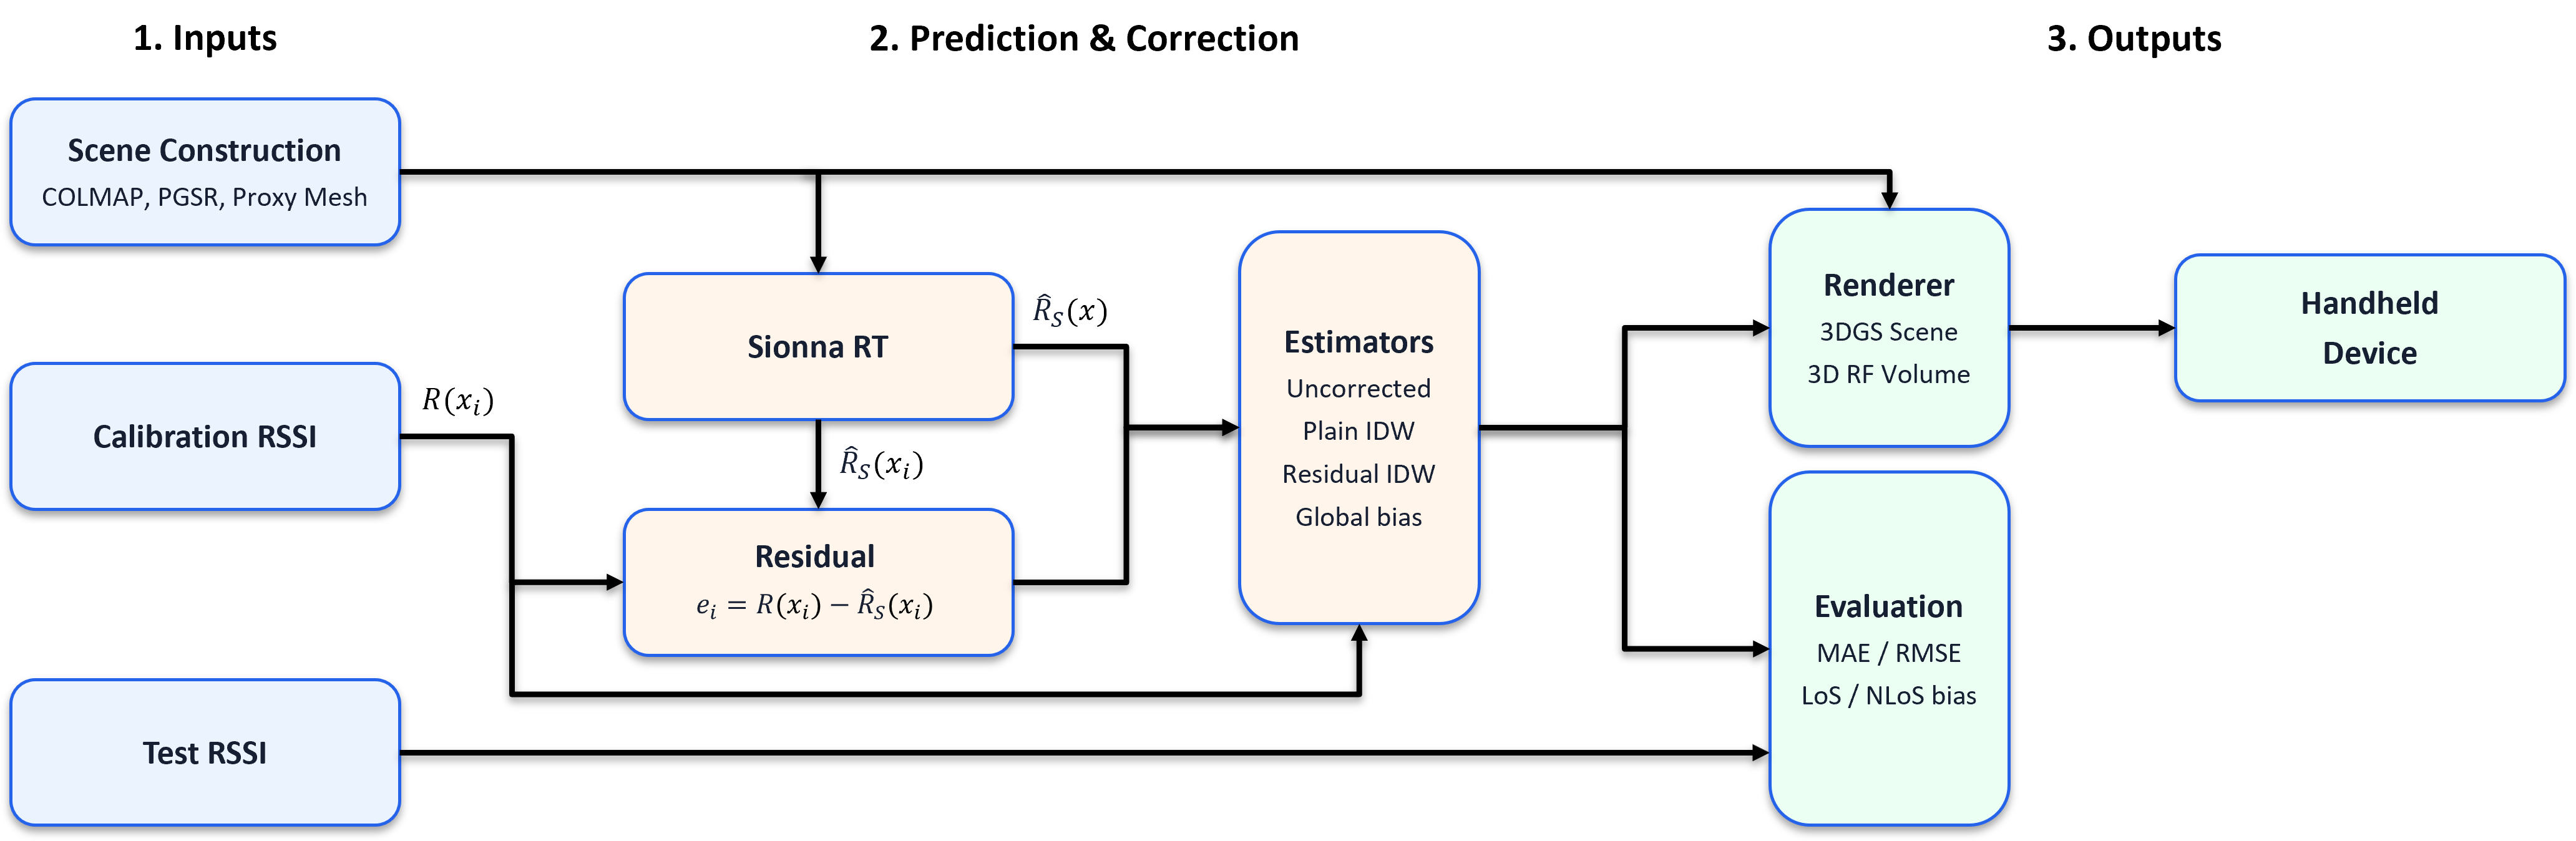
\includegraphics[width=1.0\textwidth]{paper/figure/fig1_v3.png}
  \caption{제안 파이프라인의 전체 구조. 입력, 예측 및 보정, 출력의 세 단계와 데이터 흐름.}
  \label{fig:1}
\end{figure}

그림~\ref{fig:1}의 파이프라인은 입력, 예측 및 보정, 출력의 세 단계로 구성된다. 입력 단계에서는 다중 시점 영상으로 PGSR 장면과 닫힌 프록시 메시를 같은 미터
좌표계에 구성하고, 고정 보정 노드와 이동 시험 노드의 RSSI를 수집한다. 예측 및 보정 단계에서는 Sionna RT로 예측 수신 전력 $\hat{R}_S(x)$를 계산하고,
보정 지점의 실측값과의 잔차 $e_i$를 구한 뒤 네 가지 추정 방법에 사용한다. 출력 단계에서 추정 결과는 시험 지점 RSSI와 비교해 평가하는 한편, 3DGS 장면과 함께
3차원 RF 볼륨으로 렌더러에 표시되고 핸드헬드로 전달된다. 시험 지점 RSSI는 평가에만 사용한다.

\subsection{PGSR 장면과 프록시 장면 생성}
\label{sec:3.3}

다중 시점 영상으로 COLMAP[\ref{bib:17}] 카메라 자세와 PGSR 장면을 생성한다. PGSR 메시와 실측 구조를 참고해 바닥, 천장, 벽과 주요 차폐물이 닫힌 표면을
이루도록 프록시를 구성한다. 두 장면의 관계는 그림~\ref{fig:2}와 같다.

\begin{figure}[htbp]
  \centering
  \begin{minipage}{0.48\textwidth}
    \centering
    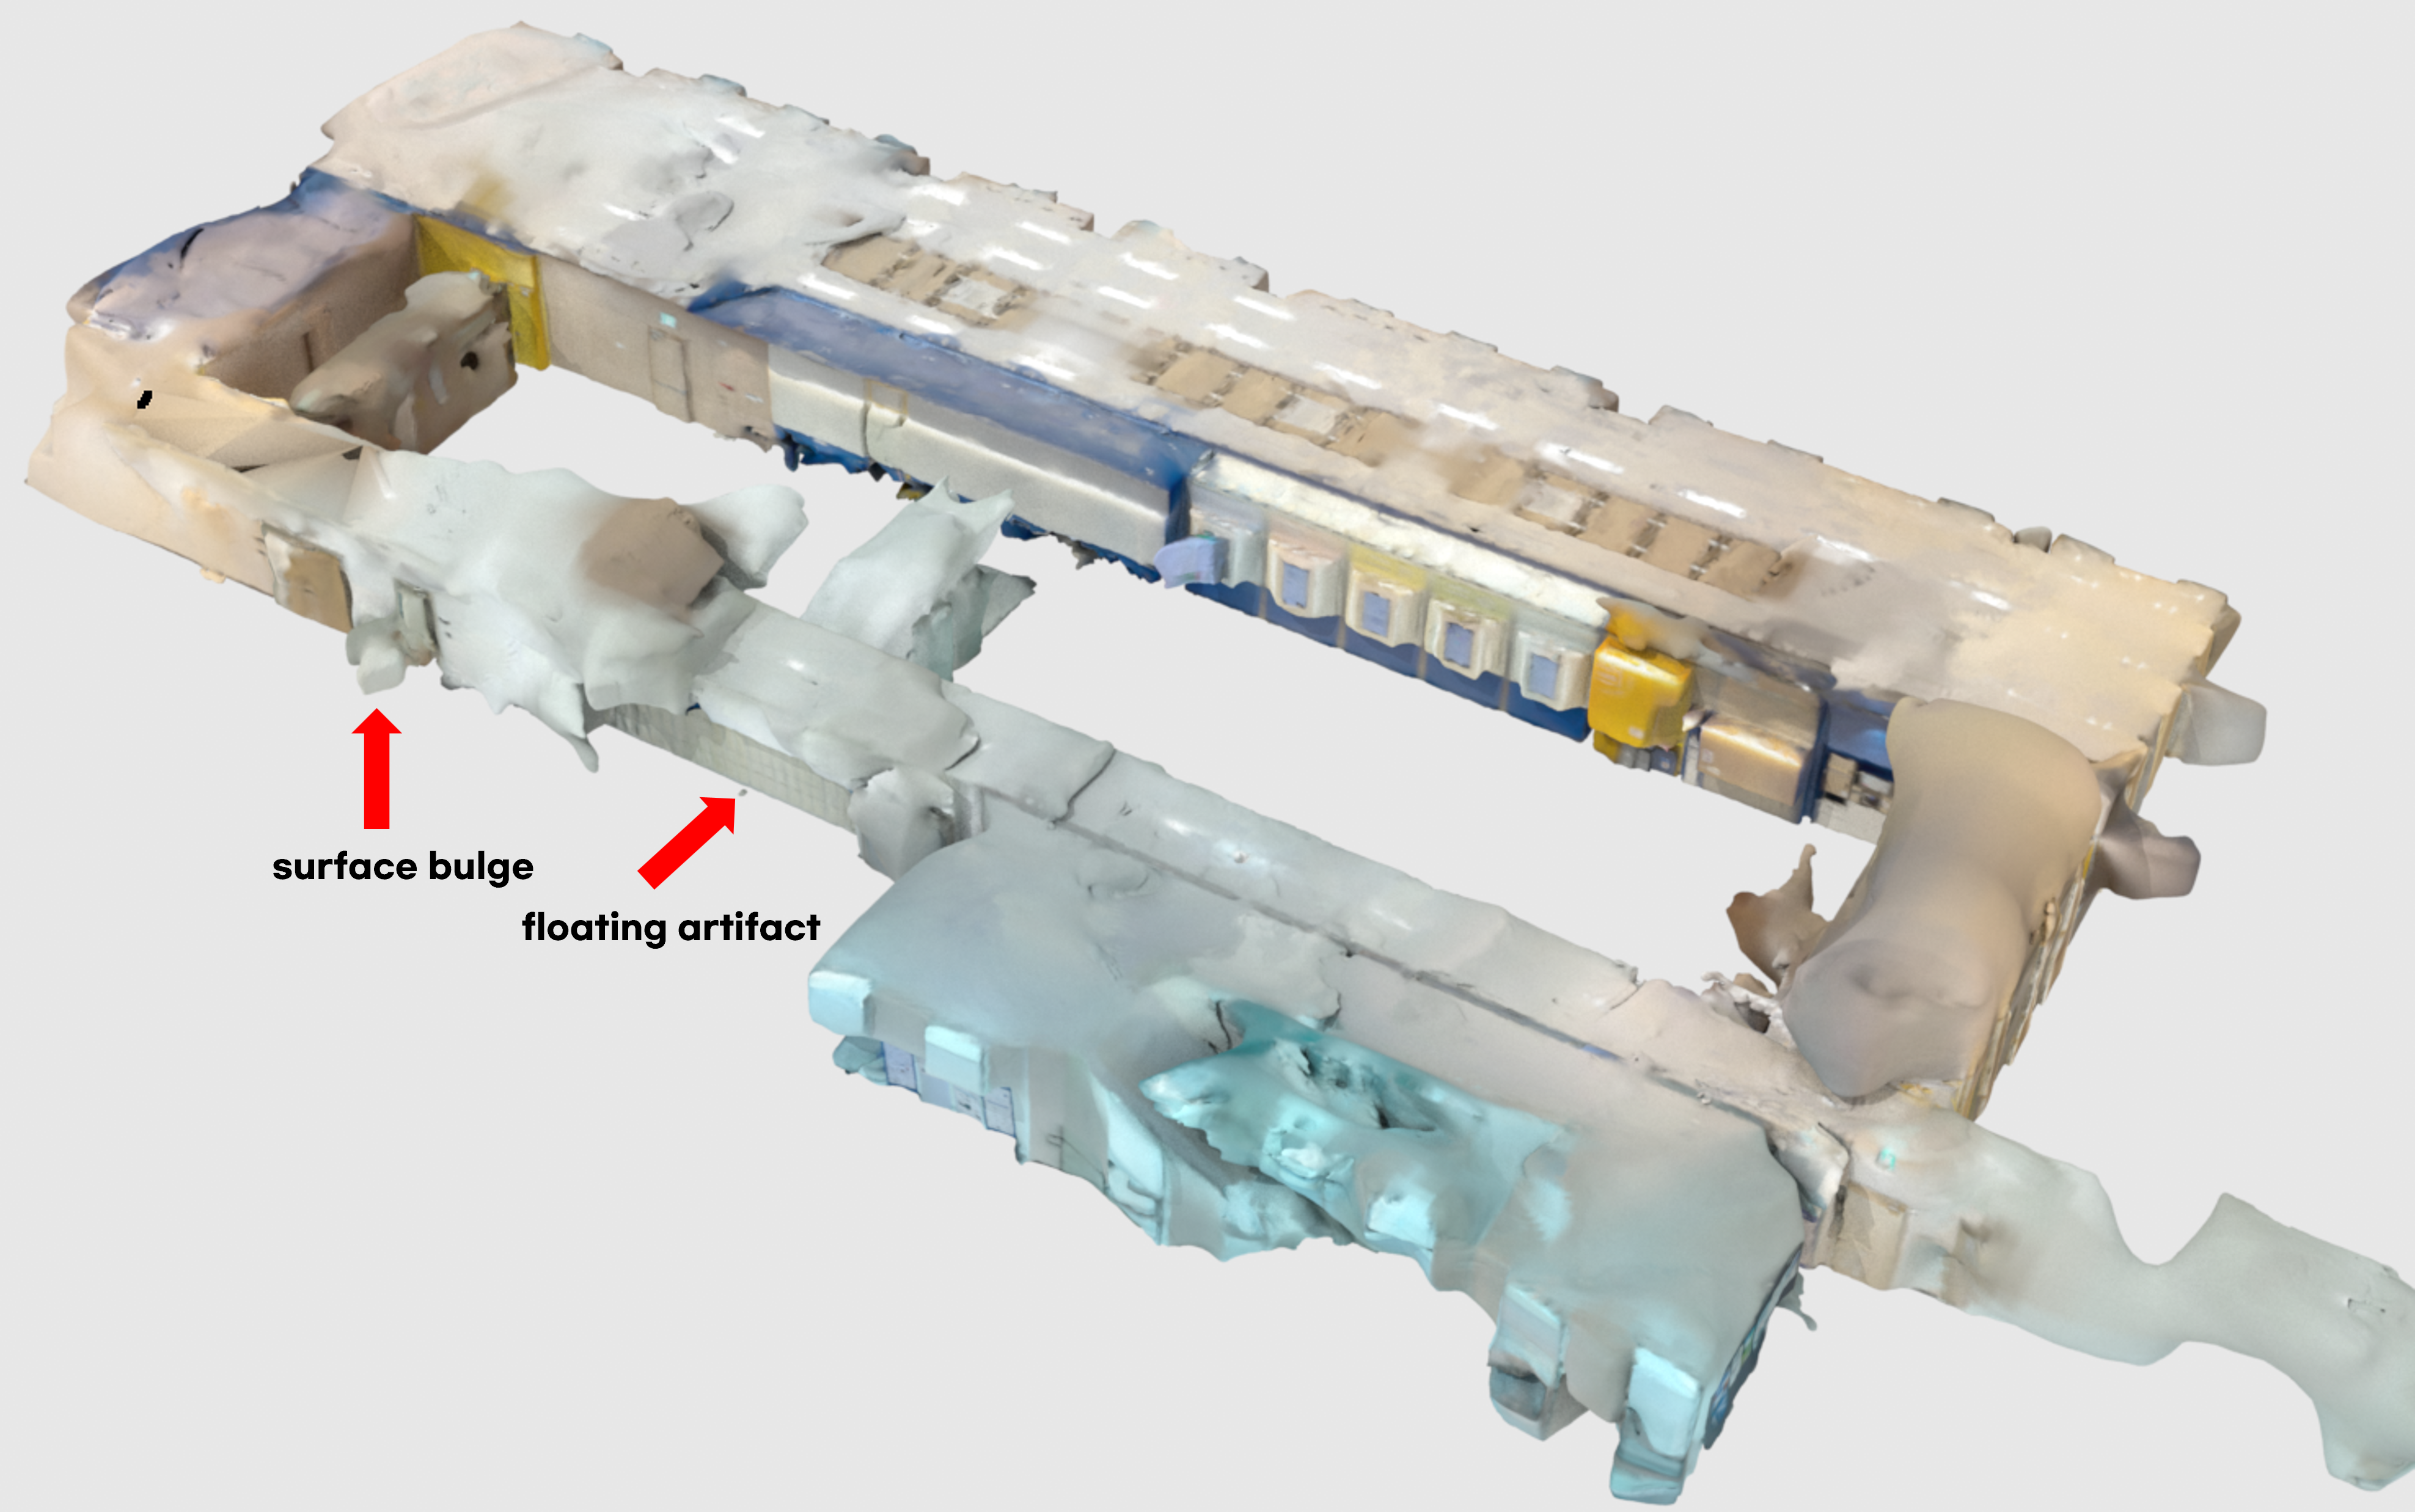
\includegraphics[width=\linewidth]{paper/figure/fig2-a_v3.png}
    \par\small (a) PGSR 표면 메시
  \end{minipage}\hfill
  \begin{minipage}{0.48\textwidth}
    \centering
    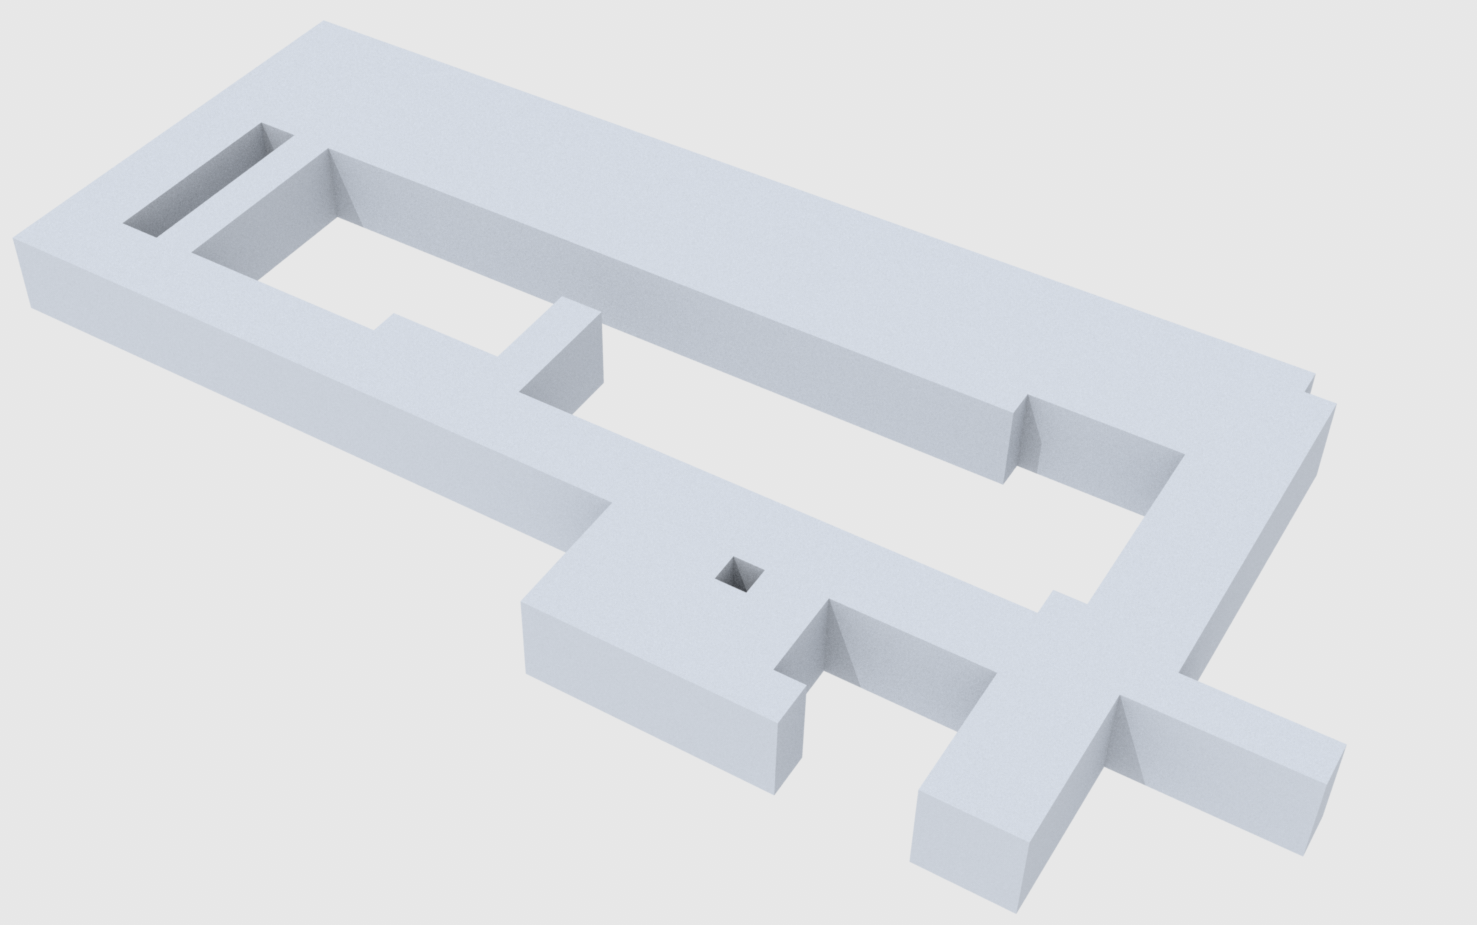
\includegraphics[width=\linewidth]{paper/figure/fig2-b_v3.png}
    \par\small (b) 닫힌 프록시 외피
  \end{minipage}
  \caption{동일 시점에서 렌더링한 장면 계층. (a) 표면 돌출과 부유 기하가 있는 PGSR 표면 메시. (b) 이로부터 생성한 바닥·벽·천장 그룹의 닫힌 프록시 외피.}
  \label{fig:2}
\end{figure}

원본 Gaussian, PGSR 메시와 프록시는 별도 계층으로 보존한다.

\subsection{Sionna RT 전파 계산}
\label{sec:3.4}

프록시 장면에는 Sionna 전파 재질을 지정한다. 2.437 GHz에서 가시선, 정반사, 회절과 확산 산란을 활성화하였다. 벽 두께와 투과손실은 실측하지 않아 벽 투과는
제외하였다. 이 설정은 코어 벽 너머 비가시선 지점의 예측 수신 전력을 낮출 수 있으므로(\ref{sec:4.4}절), 향후 재질 파라미터 측정과 함께 검증할 필요가 있다. 최대
상호작용 깊이 \texttt{max\_depth}는 예측값이 수렴하는 12로 설정하였으며, 16과 20으로 높였을 때의 추가 변화는 1\,dB 이내였다. 지점 계산은 보정 및 시험
지점의 예측 수신 전력을 생성하고, 격자 계산은 측정 높이 평면의 공간 분포를 생성한다. 두 계산은 20\,dBm 송신 전력과 단일 등방성 및 수직 편파 안테나를 가정하고
$10\log_{10}G$ 변환을 사용한다.

\subsection{RSSI 계측 경로}
\label{sec:3.5}

\subsubsection{장치 구성과 데이터 수집 경로}

계측부는 원격 ESP32 네 대와 게이트웨이 자체 측정을 합한 다섯 수신기로 구성된다. 원격 노드의 표본은
ESP-NOW[\ref{bib:18}], 게이트웨이의 UART 출력, STM32F107VCT6의 JSON 출력과 Python
Serial--MQTT 브리지를 거쳐 백엔드에 저장된다[\ref{bib:19}]. ESP32는 측정과 취합, STM32는 입력
검사와 장치별 상태 관리, PC의 브리지는 서버 연결을 담당한다. 무선 계측과 서버 연결을 분리하여 원격 노드가
서버 연결을 직접 처리하지 않도록 하였다.

구체적으로 node-01, node-03과 node-04는 각각 cal-01, cal-02와 cal-03의 고정 보정 노드,
node-02는 이동 시험 노드로 사용하였다. 게이트웨이 gw-01은 ESP-NOW 패킷을 집계하는 동시에 자체 RSSI를
측정하여 cal-04의 고정 보정 노드도 겸했다. 따라서 실험의 수신기 역할은 고정 보정 4대와 이동 시험 1대로
구성된다. 이동 노드의 위치는 고정 좌표가 아니라 시험 지점별 배정에 따라 해석한다.

그림~\ref{fig:embedded-architecture}은 계측부와 핸드헬드의 입출력 경로를 나타낸다. 계측부는 서버의
분석에 필요한 표본을 제공하고, 핸드헬드는 PC에서 생성한 영상의 표시와 자세/버튼 상태의 전달을 담당한다.

\begin{figure}[htbp]
  \centering
  \definecolor{rssiAccent}{HTML}{315D82}
  \definecolor{videoAccent}{HTML}{28776D}
  \definecolor{controlAccent}{HTML}{805B8C}
  \begin{tikzpicture}[
    panel/.style={rounded corners=4pt,line width=0.4pt},
    component/.style={draw=laneColor!75,fill=white,rounded corners=3pt,
      line width=0.65pt,text width=2.2cm,minimum height=1.05cm,
      inner xsep=3pt,inner ysep=5pt,align=center,
      font=\footnotesize,text=black!85},
    external/.style={component,dash pattern=on 3pt off 2pt},
    flow/.style={-{Latex[length=2mm,width=1.5mm]},
      draw=laneColor,line width=0.8pt},
    linklabel/.style={font=\scriptsize,text=laneColor!85!black,
      above=16pt,inner sep=1pt,align=center},
    heading/.style={anchor=west,font=\small\bfseries,text=laneColor},
    purpose/.style={anchor=east,font=\scriptsize,text=black!60}
  ]
    \begin{scope}
      \colorlet{laneColor}{rssiAccent}
      \draw[panel,draw=laneColor!20,fill=laneColor!4]
        (0,-0.85) rectangle (15.6,1.5);
      \node[heading] at (0.35,1.13) {(a) RSSI 계측 및 수집};
      \node[purpose] at (15.25,1.13) {측정 표본 → 저장·분석};
      \node[component] (remote) at (1.55,0) {\textbf{원격 ESP32}\\4대};
      \node[component] (gateway) at (4.65,0) {\textbf{게이트웨이}\\취합, 자체 측정};
      \node[component] (receiver) at (7.75,0) {\textbf{STM32}\\파싱/JSON};
      \node[component] (bridge) at (10.85,0) {\textbf{수집 PC}\\Python 브리지};
      \node[external] (storage) at (13.95,0) {\textbf{백엔드}\\저장/분석};
      \draw[flow] (remote) -- node[linklabel] {ESP-NOW} (gateway);
      \draw[flow] (gateway) -- node[linklabel] {UART} (receiver);
      \draw[flow] (receiver) -- node[linklabel] {Serial / JSON} (bridge);
      \draw[flow] (bridge) -- node[linklabel] {MQTT} (storage);
    \end{scope}

    \begin{scope}[yshift=-2.65cm]
      \colorlet{laneColor}{videoAccent}
      \draw[panel,draw=laneColor!20,fill=laneColor!4]
        (0,-0.85) rectangle (15.6,1.5);
      \node[heading] at (0.35,1.13) {(b) 영상 수신 및 표시};
      \node[purpose] at (15.25,1.13) {완성 영상 → 단말 화면};
      \node[external] (source) at (1.55,0) {\textbf{PC/중계 서버}\\완성 영상 제공};
      \node[component] (handheld) at (7.75,0) {\textbf{ESP32-S3}\\영상 수신/변환};
      \node[component] (display) at (13.95,0) {\textbf{NT35510 LCD}\\$800\times480$};
      \draw[flow] (source) -- node[linklabel] {TCP} (handheld);
      \draw[flow] (handheld) -- node[linklabel] {병렬 버스} (display);
    \end{scope}

    \begin{scope}[yshift=-5.3cm]
      \colorlet{laneColor}{controlAccent}
      \draw[panel,draw=laneColor!20,fill=laneColor!4]
        (0,-0.85) rectangle (15.6,1.5);
      \node[heading] at (0.35,1.13) {(c) 자세·버튼 상태 전달과 제어};
      \node[purpose] at (15.25,1.13) {입력 상태 → 뷰어 반영};
      \node[component] (sensor) at (1.55,0) {\textbf{BNO085}\\버튼 2개};
      \node[component] (control) at (5.68,0) {\textbf{ESP32-S3}\\입력 상태 전송};
      \node[external] (backend) at (9.82,0) {\textbf{백엔드}\\입력 검증 및 중계};
      \node[external] (viewer) at (13.95,0) {\textbf{PC 뷰어}\\입력 반영};
      \draw[flow] (sensor) -- node[linklabel] {I2C·GPIO} (control);
      \draw[flow] (control) -- node[linklabel] {UDP} (backend);
      \draw[flow] (backend) -- node[linklabel] {WebSocket} (viewer);
    \end{scope}
  \end{tikzpicture}
  \caption{임베디드 계측 및 단말 입출력 경로. (a) RSSI 계측 및 수집,
  (b) 영상 수신 및 표시, (c) 자세/버튼 상태 전달과 제어. 점선 상자는 백엔드와 PC 측 구성요소이며,
  동일한 ESP32-S3를 영상 수신과 입력 전송 경로에 나누어 표기하였다.}
  \label{fig:embedded-architecture}
\end{figure}


\subsubsection{RSSI 취득과 패킷 검사}

최종 실험은 채널 6(2.437\,GHz)에서 수행하였다. 원격 노드는 RSSI 취득 간격을 200\,ms,
전송 간격을 1{,}000\,ms로 설정하고, 최근 유효 표본 최대 다섯 개의 이동평균을 약 1초 간격으로 전송한다.
게이트웨이 자체 측정은 취득 및 보고 간격을 1{,}000\,ms로 설정하며, 동일하게 최근 유효 표본 최대
다섯 개를 평균한다. 이 간격은 설정값으로, 실제 취득 및 전송 간격은 처리 시간과 스케줄링에 따라 달라질 수 있다.
유효 범위는
$-110\leq\mathrm{RSSI}\leq-10$\,dBm이며, 약한 신호가 수집 계층에 따라 다르게 제거되지 않도록
하한을 통일하였다. 필터링 RSSI는 내부에서 dBm 값의 10배인 정수로 표현하며, STM32에서 서버로 전달할
때는 정수 dBm으로 반올림한다.

원격 노드는 측정값과 장치 식별 및 오류 정보를 함께 전송한다. 게이트웨이는 전송 오류를 검사하고 자체
측정값도 함께 UART로 STM32에 전달한다. STM32의 수신 인터럽트에서는 바이트만 링 버퍼에 저장하고,
행 파싱과 JSON 생성은 메인 루프에서 수행한다. STM32는 수신 자료를 검증한 뒤 장치별 최신 상태를 갱신한다.

브리지는 장치별 자료를 백엔드로 전달하며, 이후의 수집, 검증, 저장은 \ref{sec:network}절에서 다룬다.
대상 AP의 식별 정보는 서버까지 전달되지 않으므로, 실험 전에 측정 대상과 채널을 고정하고 기록하였다.

\subsubsection{장치 편차 보정과 시간 기준}

장치별 편차는 실험 전 다섯 장치를 같은 위치에 두고 동시에 측정하여 산출한다. 장치 $k$가 보고한
이동평균 RSSI 시계열의 중앙값을 $m_k$라 하고, 다섯 장치의 $m_k$에 대한 중앙값을 $\bar{m}$이라 하자.
장치 $k$의 보정값 $b_k$와 편차 보정 후 측정값은 다음과 같다.
\[
  \bar{m}=\operatorname{median}_{k=1,\ldots,5}m_k,\qquad
  b_k=\bar{m}-m_k,\qquad
  R_k^{\mathrm{corr}}(t)=R_k(t)+b_k.
\]
여기서 $R_k(t)$는 펌웨어의 이동평균 처리를 거친 장치 편차 보정 전 RSSI이며 $b_k$의 단위는 dB이다. 특정 장치 하나가 아니라 전체
중앙값을 기준으로 사용하여 기준 장치의 이상치 영향을 줄인다. 이 절차는 장치 사이의 상대 편차를 맞추는
것으로, 절대 전력 교정은 아니다. 본 실험에서는 실험 전 보정값을 사용하였으며, 실험 후 장치 편차를 다시
측정하지 않았다.

원격 노드와 게이트웨이는 SNTP로 맞춘 측정 시각을 표본마다 함께 전송하고, 동기화 전의 표본은 시각 무효
플래그로 구분한다. 백엔드는 이 노드 측정 시각과 서버 수신 시각을 별도 열로 저장한다. 정지 측정의 시험 구간
배정과 실시간 경로의 시간창에서 두 시각을 사용하는 방법은 \ref{sec:network}절과 \ref{sec:3.6}절에서 설명한다.

\subsection{백엔드 수집 및 저장, 실시간 중계}
\label{sec:network}

백엔드는 계측 자료의 수집, 저장과 분석 준비를 담당하고, 핸드헬드와 렌더러 사이의 실시간 연동을 지원한다.
서버별 역할과 연결 구조는 그림~\ref{fig:serverarch}와 같다.

\begin{figure}[htbp]
  \centering
  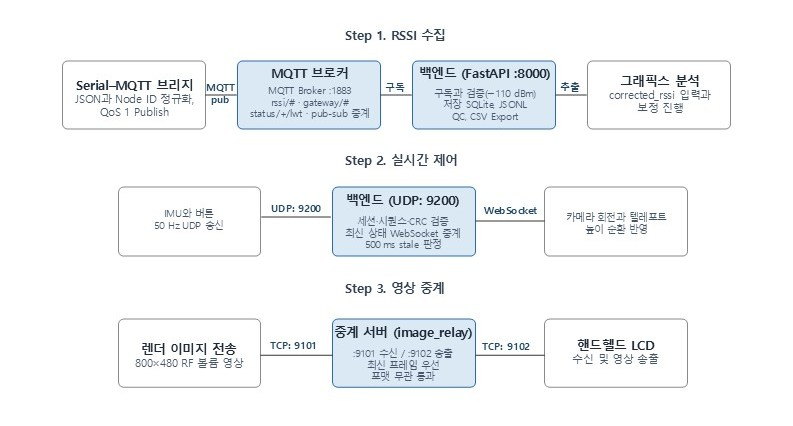
\includegraphics[width=\textwidth]{Network_Backend/Server_com.jpg}
  \caption{서버 구성과 포트 및 역할, 과정별 연결(Step 1. RSSI 수집, Step 2. 실시간 제어, Step 3. 영상 중계).}
  \label{fig:serverarch}
\end{figure}

\subsubsection{중앙 수집과 데이터 검증}

백엔드는 MQTT로 다섯 수신기의 표본과 접속 상태를 수집한다. 측정 자료의 형식을 통일하고 RSSI 범위와
오류 상태를 검사한다. 비정상 표본은 제외 사유와 함께 보존하되 분석에서는 제외하며, 패킷 순번으로 중복과
누락을 확인한다. 수신 및 저장 성공만으로 앞단 무선과 UART 구간의 무손실 전달을 보장하지는 않는다.
각 표본에는 노드가 보낸 측정 시각과 백엔드가 기록한 서버 수신 시각을 함께 저장한다. 두 시각의 차이가 허용 범위를
크게 벗어나면 노드 시계가 맞지 않은 것으로 보고 서버 수신 시각을 사용한다.

\subsubsection{저장과 실험 관리}

수신 원본과 분석용 자료를 분리하여 저장하고, 해석할 수 없는 메시지도 가능한 범위에서 원문을 보존한다.
자료는 실험과 측정 구간 단위로 관리하며, 각 표본을 해당 시험 지점의 기록 구간에 배정한다.

\subsubsection{품질 검사와 내보내기}

자료를 전달하기 전에 채널, RSSI 범위, 오류 상태와 표본 수를 검사하고 좌표 및 장치 편차 보정값의
누락 여부를 확인한다. 이후 측정 원본, 지점별 대표값, 송신 및 수신 좌표와 보정값을 분석용 자료로 정리하여
전달한다. RF 추정 및 시각화에는 장치 편차를 반영한 보정 RSSI를 사용한다.
노드 상태와 수집 현황은 실시간 모니터링 화면에서 확인할 수 있다(그림~\ref{fig:monitor}).

\begin{figure}[htbp]
  \centering
  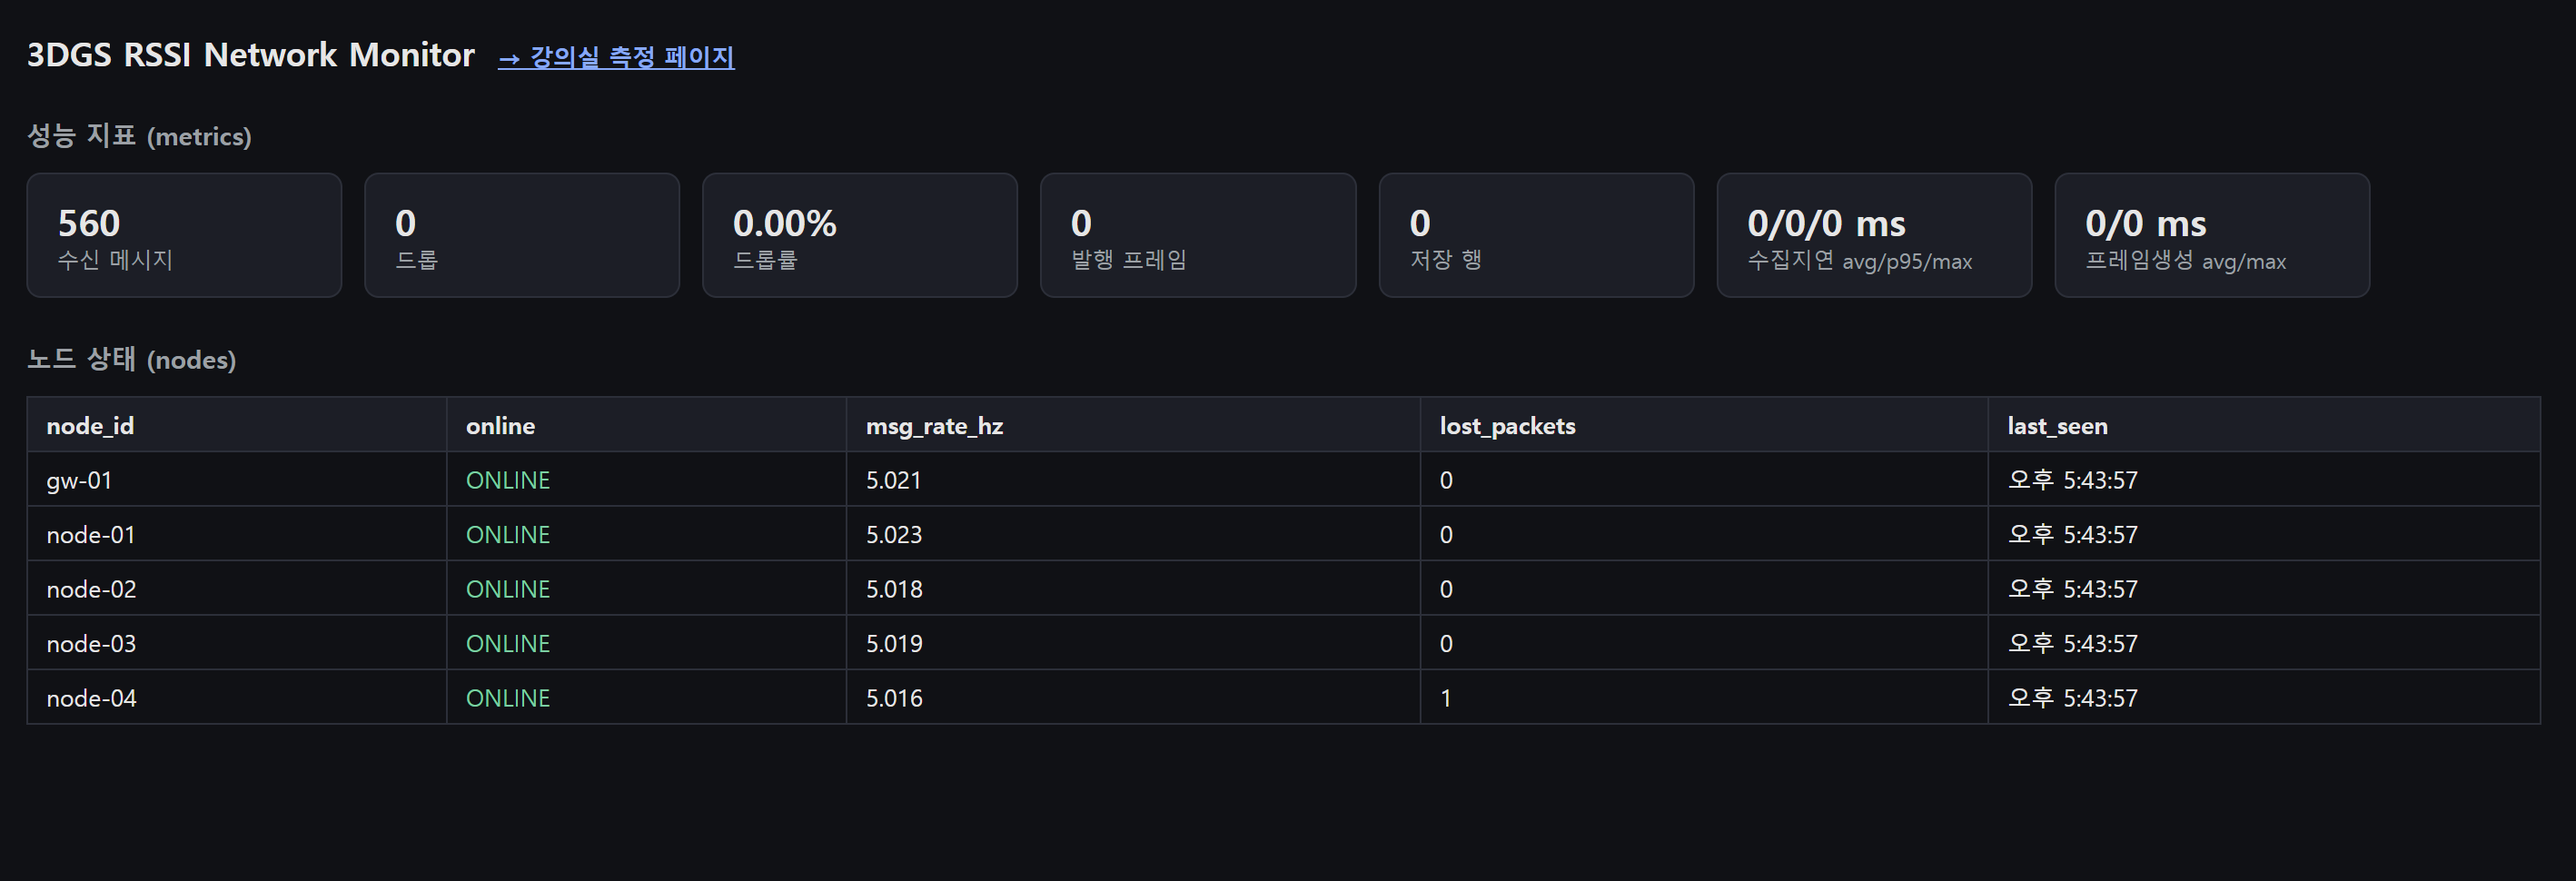
\includegraphics[width=\textwidth]{Network_Backend/monitoring_sys.png}
  \caption{백엔드 실시간 모니터링 화면 예시(노드 상태와 수집 현황).}
  \label{fig:monitor}
\end{figure}

\subsubsection{실시간 제어와 영상 중계}

실시간 경로는 측정 데이터의 저장 및 분석과 독립적으로 동작한다. 백엔드는 핸드헬드가 보낸 자세와 버튼
입력의 유효성과 순서를 검사하고, 최신 상태를 렌더러에 중계한다. 일정 시간 갱신이 없으면 오래된 상태로
표시한다. 영상 중계 서버는 프레임을 검사한 뒤 재인코딩 없이 최신 영상을 우선 전달한다.

실시간 RSSI 프레임은 여러 노드의 값을 200\,ms 시간창으로 묶어 WebSocket으로 전달한다. 중간 단계에는 서버 도착
시각으로 창을 나누었으나, 수집 지연의 p95(244\,ms)가 창 길이를 넘어 같은 프레임의 값이 서로 다른 측정 구간에
속할 수 있었다. 이에 노드 측정 시각을 기준으로 창을 나누고, 창이 끝난 뒤에도 300\,ms의 유예 구간 동안 늦게
도착한 표본을 기다린 뒤 프레임을 확정하도록 바꾸었다. 확정 시점은 측정 시각 워터마크로 판단하며, 입력이 멈추면
서버 시계를 기준으로 창을 닫아 프레임이 무기한 대기하지 않게 하였다. 유예 구간이 지난 뒤 도착한 표본은 별도로
집계한다.

백엔드와 영상 중계 서버의 동작 상태는 그림~\ref{fig:serverstate}과 같다.

\begin{figure}[htbp]
  \centering
  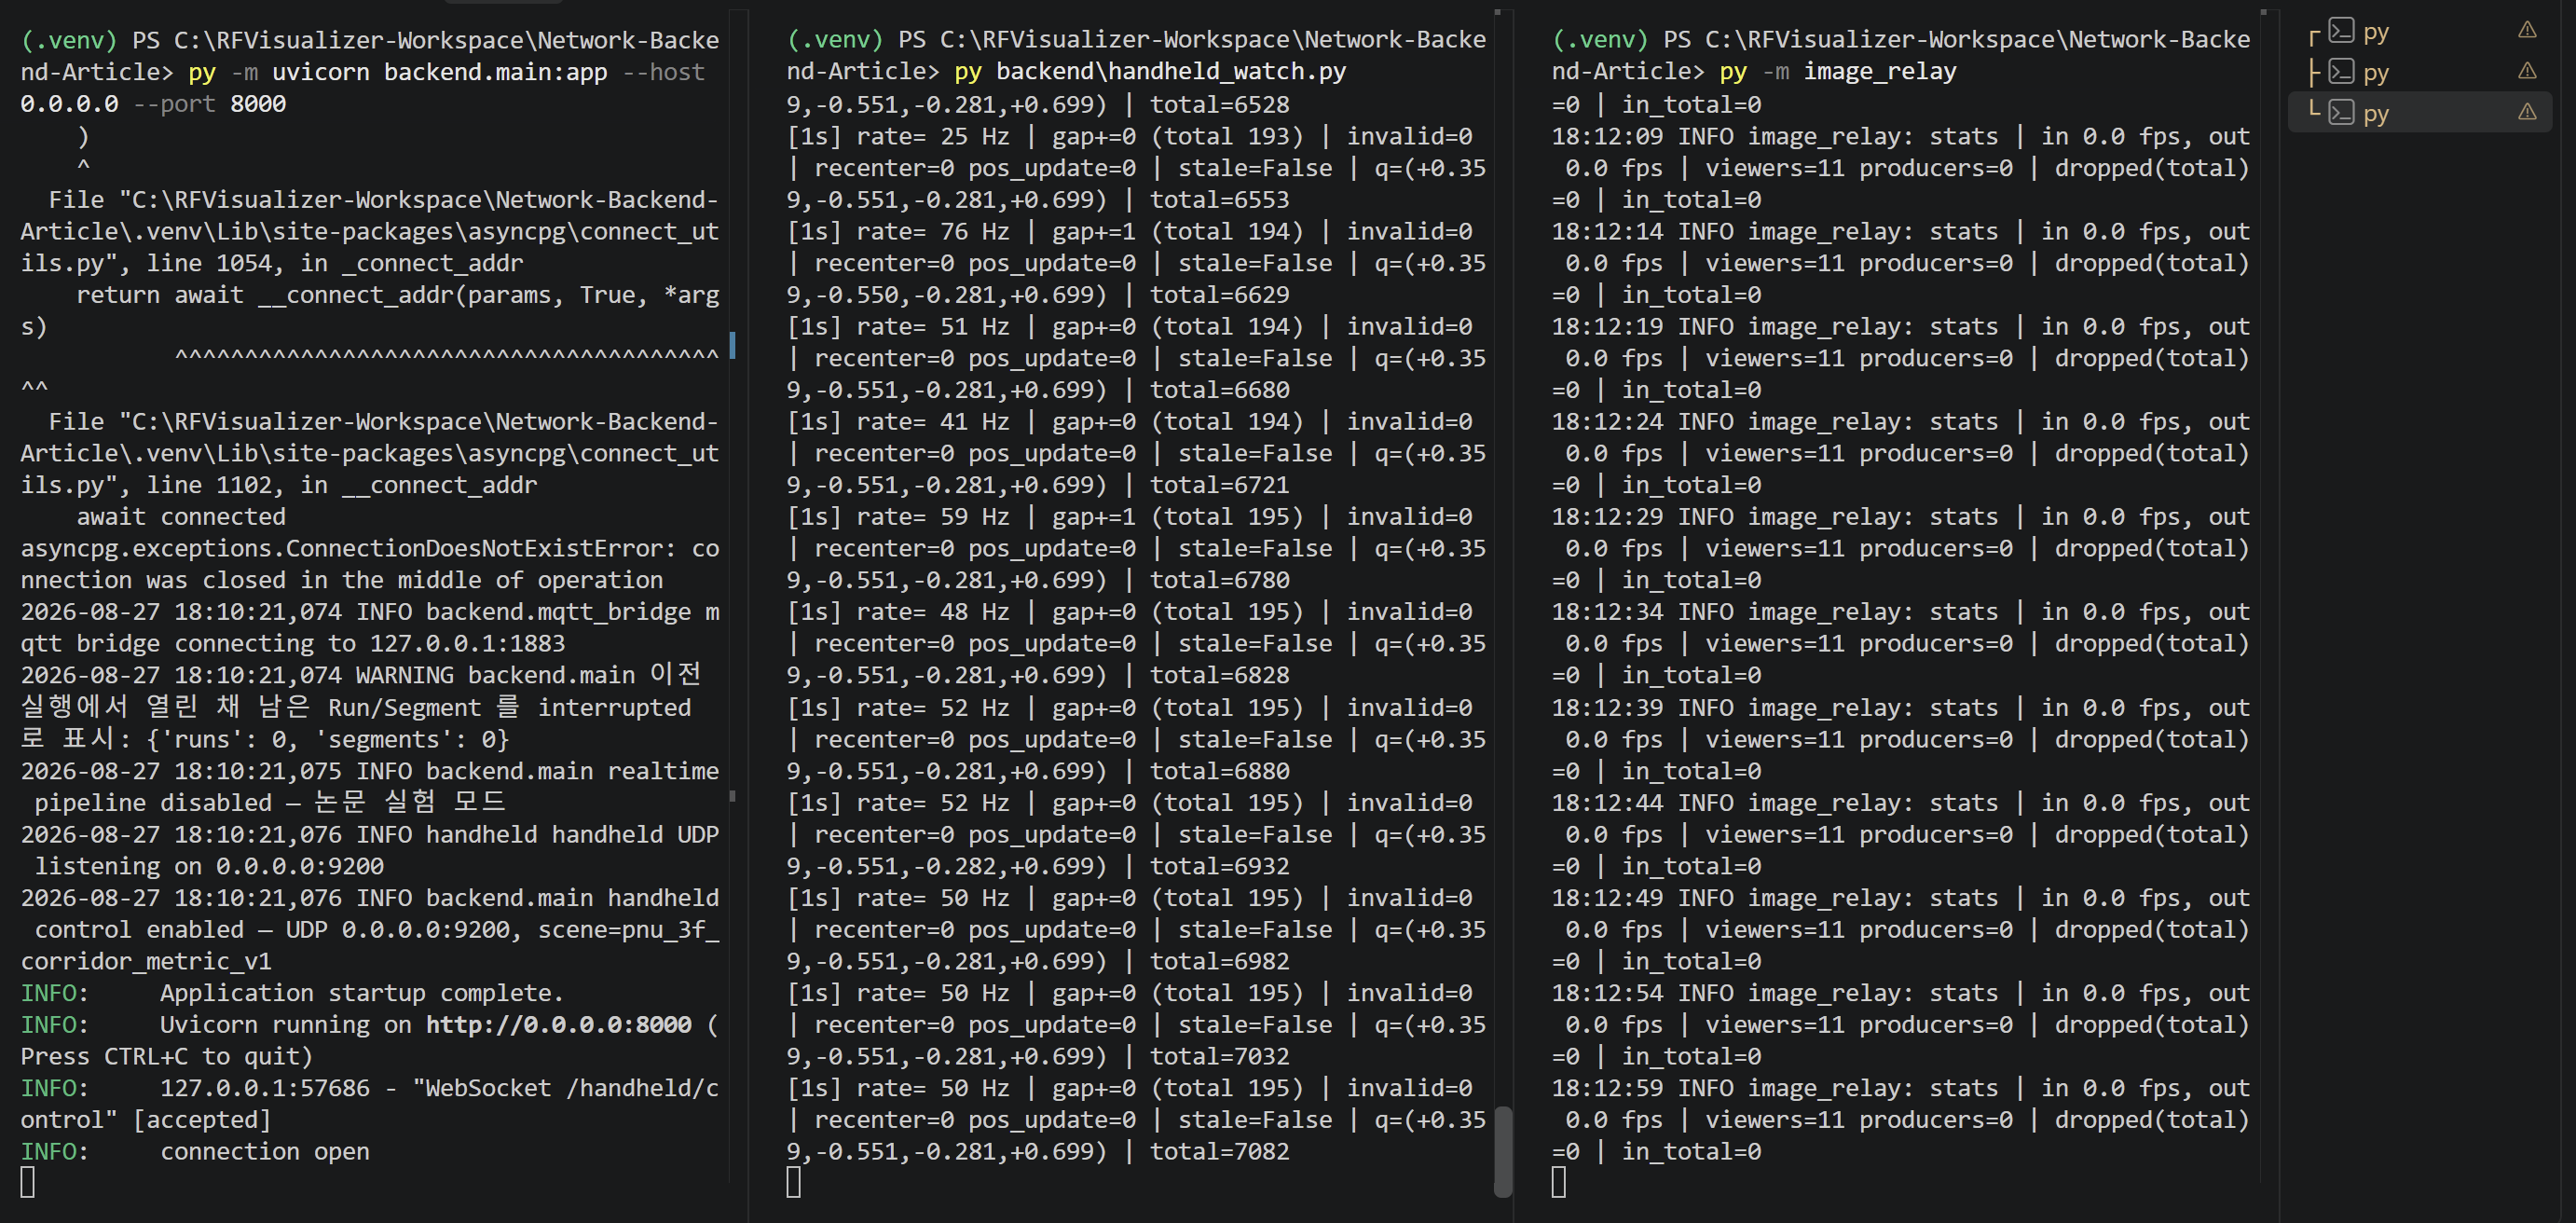
\includegraphics[width=\textwidth]{Network_Backend/image_relay.png}
  \caption{실시간 경로 구성 서버(백엔드 및 상태 확인 도구, 중계 서버)의 동작 상태.}
  \label{fig:serverstate}
\end{figure}

\subsection{실측값과 시뮬레이션의 결합}
\label{sec:3.6}

보정 위치를 $x_i$라 할 때 IDW 가중치는 식~\eqref{eq:2}와 같다. 지수 $p=2$는 평가 전에 고정했고, $\epsilon=10^{-12}$는 0으로 나눗셈을
방지하는 상수다. 질의 위치가 보정 위치와 일치하면 해당 표본을 직접 사용한다.

\begin{equation}
  \label{eq:2}
  w_i(x)=\frac{1}{\lVert x-x_i\rVert_2^p+\epsilon}.
\end{equation}

보정 RSSI를 $R_i=R(x_i)$라 할 때 비교하는 네 방법은 다음과 같다. \textbf{원시 예측}(uncorrected prediction)은 실측 보정 없이
$\hat{R}_S(x)$를 그대로 사용한다. \textbf{일반 IDW}(plain IDW)는 $R_i$를 식~\eqref{eq:2}의 가중치로 평균한다. \textbf{잔차
IDW}(residual IDW)는 식~\eqref{eq:1}의 $e_i$를 보간하여 시뮬레이션 예측에 더한다(식~\eqref{eq:3}). \textbf{전역 편향
보정}(global-bias correction)은 같은 잔차의 산술평균을 모든 예측에 더한다(식~\eqref{eq:4}).

\begin{equation}
  \label{eq:3}
  \hat{R}_{hybrid}(x)=\hat{R}_S(x)+\frac{\sum_i w_i(x)e_i}{\sum_i w_i(x)}.
\end{equation}

\begin{equation}
  \label{eq:4}
  \hat{R}_{global}(x)=\hat{R}_S(x)+\frac{1}{N}\sum_{i=1}^{N}e_i.
\end{equation}

여기서 $N$은 보정 지점 수다. 네 방법은 같은 보정/시험 분할과 좌표를 사용한다. 공간 구조는 $\hat{R}_S$를 계산하는 Sionna RT 단계에서 반영되며, 잔차 보간은
보정 지점이 네 개뿐인 조건을 고려해 유클리드 거리 기반 IDW로 단순화하였다.

각 시험 지점의 기록 시간창은 \textbf{백엔드 서버 수신 시각}을 기준으로 정의하고, 같은 시간창에 수신된
고정 보정 자료로 잔차 $e_i$를 계산한다. 보정값의 시간 변화를 반영하기 위해 실행 전체 평균 대신 시간창별
값을 사용한다. 정지 측정은 지점마다 120\,s의 긴 기록창을 사용하므로, 표본의 구간 배정에는 서버 수신 시각을
사용하였다. 연속 측정 회차에서 노드 측정 시각과 서버 수신 시각의 차이는 p95 기준 0.46 $\sim$ 0.71\,s였다
(\ref{sec:4.6}절). 이 차이는 기록창 길이의 0.6\,\% 이하이며, 기록창 경계에서 일부 표본이 인접 구간으로 넘어갈 수
있는 정도이다. 서버 수신 시각은 노드 시계의 동기화 실패에 영향을 받지 않으며, 노드 측정 시각도 함께 저장하므로
필요하면 측정 시각 기준으로 다시 배정할 수 있다.

\subsection{3차원 RF 볼륨과 시각화}
\label{sec:3.7}

방법별 예측을 여러 높이의 격자로 다시 계산해 0.25 m에서 2.75 m까지 여섯 높이의 3차원 RF 볼륨으로 묶는다. 각 높이의 격자는 같은 XY 해상도를 공유하며, 전파
계산이 실패했거나 정의되지 않은 위치는 유효성 마스크로 구분한다.

렌더러는 이 볼륨을 3차원 텍스처로 불러와 광선 행진(ray marching)으로 알파 합성한다. 프록시 메시의 깊이보다 먼 샘플은 제거하여 벽 뒤 신호의 표시를 제한한다.
렌더러는 평가한 네 방법 중 전역 편향 보정을 제외한 원시 예측, 일반 IDW와 잔차 IDW의 세 RF 볼륨을 같은 시점에서 전환할 수 있다.

다만 실측 잔차는 측정이 이루어진 단일 높이에서만 존재하므로 다른 높이의 잔차 보정값은 수직 외삽값이다. 따라서 RF 볼륨의 수직 변화는 정성적 시각화로 한정하고, 정량 평가는
실측 높이 평면에서만 수행한다.

\subsection{핸드헬드 인터페이스와 영상 전송}
\label{sec:3.8}

\subsubsection{단말 하드웨어와 역할 분담}

핸드헬드는 ESP32-S3, BNO085 IMU, LCD와 두 개의 물리 버튼으로 구성된다. 제어기는 16\,MB 플래시와
8\,MB PSRAM을 갖추고, NT35510 기반의 물리 해상도 $480\times800$ LCD를 가로 방향
$800\times480$으로 구동한다. LCD는 16-bit 8080형 병렬 버스(I80)로 연결하였다. 3DGS 렌더링과 RF 볼륨
합성은 PC에서 수행하고, 핸드헬드는 완성된 영상을 수신 및 검증하고 디코딩과 색 변환을 거쳐 표시하는 씬 클라이언트
(thin client)로 동작한다. 단말은 자세와 버튼 상태도 전송하므로, 임베디드 장치에서 장면을 다시 계산하지
않고 PC의 시각화 결과를 현장에서 탐색할 수 있다. 실물 외관은 그림~\ref{fig:8}에 제시한다.

\subsubsection{영상 프레임 수신과 JPEG 처리}

본 시스템의 영상 송신 구성에서는 렌더러가 $800\times480$ 프레임을 Baseline JPEG로 인코딩해 전송한다.
각 프레임에는 순번, 생성 시각과 페이로드 길이를 포함한 RFJF 공통 헤더를 붙이고, 형식 필드를
\texttt{flags=0}으로 지정한다.
네트워크 중계기는 프레임을 다시 인코딩하지 않고 단말에 전달한다.

단말은 TCP 스트림에서 필요한 길이만큼 반복 수신하여 헤더와 페이로드를 조립한다. TCP 읽기 한 번을
프레임 하나로 간주하지 않으며, 식별자, 버전, 형식, 길이를 검사하고 단말의 수신 상한을 넘는 프레임은
거부한다. 중계 규격의 페이로드 상한은 8\,MiB이고, 단말 설정의 수신 상한은 512\,KiB이다.

수신한 JPEG는 RGB565 영상으로 디코딩한다. 이어서 RGB565 전용 색 변환 조회표를 이용해
RGB666 데이터를 I80 전송 형식으로 패킹하고, 직접 메모리 접근(DMA)으로 LCD에 출력한다.
단말의 대기 프레임 관리와 LCD DMA 출력 구조는 다음 절에서 설명한다.

\subsubsection{프레임 버퍼와 LCD DMA 출력}

압축 프레임 저장에는 512\,KiB PSRAM 버퍼 두 개를 사용하며, 출력 대기 큐에는 완성 프레임이 저장된
버퍼의 참조를 최대 한 개 보관한다. 수신 버퍼 확보 또는 완성 프레임 전달 시 필요에 따라 기존 대기
프레임을 폐기하고 최신 프레임을 우선 처리하여 오래된 화면의 누적을 제한한다. 이러한 의도적 교체는
네트워크 전송 손실과 구분한다.

JPEG 디코딩 결과는 압축 버퍼와 별도로 PSRAM에 할당한 RGB565 프레임 버퍼 한 개에 저장한다.
이 버퍼의 크기는 $800\times480\times2=768{,}000$\,byte이다.
버퍼 흐름은 그림~\ref{fig:embedded-buffer-flow}과 같다.

\begin{figure}[htbp]
  \centering
  \definecolor{bufferReceive}{HTML}{315D82}
  \definecolor{bufferOutput}{HTML}{28776D}
  \begin{tikzpicture}[
    panel/.style={rounded corners=4pt,line width=0.4pt,
      draw=laneColor!20,fill=laneColor!4},
    stage/.style={draw=laneColor!75,fill=white,rounded corners=3pt,
      line width=0.65pt,text width=2.7cm,minimum height=1.45cm,
      inner xsep=3pt,inner ysep=5pt,align=center,
      font=\footnotesize,text=black!85},
    memory/.style={stage,text width=3.2cm},
    slot/.style={draw=laneColor!45,fill=laneColor!8,rounded corners=2pt,
      text width=1.05cm,minimum height=0.45cm,inner sep=2pt,
      align=center,font=\scriptsize,text=laneColor!85!black},
    flow/.style={-{Latex[length=2mm,width=1.5mm]},
      draw=laneColor,line width=0.8pt},
    linklabel/.style={above=5pt,font=\scriptsize,
      text=laneColor!85!black,align=center,inner sep=1pt},
    heading/.style={anchor=west,font=\small\bfseries,text=laneColor},
    note/.style={font=\scriptsize,text=black!65,align=center}
  ]
    \begin{scope}
      \colorlet{laneColor}{bufferReceive}
      \draw[panel] (0,-1.25) rectangle (15.6,2.0);
      \node[heading] at (0.35,1.62) {(a) 프레임 수신 및 대기};
      \node[stage] (receive) at (2,0)
        {\textbf{수신 태스크}\\[3pt]프레임 조립/검증};
      \node[memory] (compressed) at (7.8,0) {};
      \node[font=\footnotesize\bfseries,text=black!85] at (7.8,0.4) {PSRAM};
      \node[slot] at (7.05,-0.22) {압축 A};
      \node[slot] at (8.55,-0.22) {압축 B};
      \node[stage] (ready) at (13.6,0)
        {\textbf{출력 대기 큐}\\[3pt]압축 버퍼 참조 \textbf{1개}};
      \draw[flow] (receive) -- node[linklabel] {압축 프레임 저장} (compressed);
      \draw[flow] (compressed) -- node[linklabel] {완성 프레임 참조} (ready);
      \node[note] at (2,-0.98) {TCP 스트림 → RFJF 프레임};
      \node[note] at (7.8,-0.98) {압축 프레임 버퍼 2개};
    \end{scope}

    \begin{scope}[yshift=-3.85cm]
      \colorlet{laneColor}{bufferOutput}
      \draw[panel] (0,-3.8) rectangle (15.6,2.0);
      \node[heading] at (0.35,1.62) {(b) JPEG 디코딩 및 LCD 출력};
      \node[stage] (decode) at (13.6,0)
        {\textbf{JPEG 디코딩}\\[3pt]RGB565 영상 생성};
      \node[memory] (rgbframe) at (7.8,0)
        {\textbf{PSRAM RGB565}\\[3pt]프레임 버퍼 1개\\768,000\,byte};
      \node[stage] (packing) at (2,0)
        {\textbf{스트라이프 패킹}\\[3pt]RGB666 색 변환\\I80 패킹};
      \node[memory] (dma) at (2,-2.6) {};
      \node[font=\footnotesize\bfseries,text=black!85] at (2,-2.2) {내부 RAM};
      \node[slot] at (1.25,-2.82) {DMA A};
      \node[slot] at (2.75,-2.82) {DMA B};
      \node[stage] (lcd) at (7.8,-2.6)
        {\textbf{NT35510 LCD}\\[3pt]스트라이프 출력};
      \draw[flow] (decode) -- node[linklabel] {디코딩 결과 저장} (rgbframe);
      \draw[flow] (rgbframe) -- node[linklabel] {디코딩 완료 후} (packing);
      \draw[flow] (packing.south) -- (dma.north);
      \draw[flow] (dma) -- node[linklabel] {DMA 교대 전송} (lcd);
      \node[note] at (7.8,-3.57) {$800\times480$ 화면};
      \node[note] at (2,-3.57) {버퍼당 $800\times16$ 픽셀};
    \end{scope}

    \draw[-{Latex[length=2mm,width=1.5mm]},draw=bufferReceive,
      line width=0.8pt] (ready.south) --
      node[right=5pt,font=\scriptsize,text=black!65] {참조 인계} (decode.north);
    \node[note,text width=15cm] at (7.8,-8.05)
      {\textbf{DMA 버퍼 재사용 조건}\quad DMA 전송 완료 확인 후 재사용};
  \end{tikzpicture}
  \caption{최신 프레임 우선 처리와 이중 버퍼 출력 구조.
  (a) 대기 큐는 PSRAM 압축 버퍼를 참조하며 최신 프레임을 우선 처리한다.
  (b) JPEG를 별도의 PSRAM RGB565 프레임으로 디코딩한 뒤 스트라이프를 패킹하고,
  내부 RAM의 DMA 이중 버퍼로 LCD에 출력한다.}
  \label{fig:embedded-buffer-flow}
\end{figure}

LCD 출력에는 내부 RAM의 $800\times16$픽셀 DMA 버퍼 두 개를 사용한다. JPEG 디코딩을 완료한 뒤
LCD 출력을 시작하며, 출력 단계에서는 다음 16행의 픽셀을 LCD 전송 형식으로 패킹하는 작업과 현재
스트라이프의 DMA 전송을 중첩한다. BNO085의 I2C 처리와 LCD 전송이 겹치지 않도록 두 작업의 실행
구간을 공통 뮤텍스로 조정한다. DMA 완료 대기가 시간 초과되면 전송 중인 버퍼의 재사용을 막기 위해
단말을 재부팅한다.

\newpage
\subsubsection{IMU 자세와 버튼 상태 전달}

BNO085의 Game Rotation Vector를 I2C로 취득하고 자세와 두 버튼의 현재 상태를 약 50\,Hz로 백엔드에
전송하도록 설정하였다. 자세는 Euler 각 대신 네 성분의 쿼터니언 $(x,y,z,w)$로 전달하며, 모든 성분이
유한하고 노름이 $0.97\sim1.03$인 경우에 패킷의 자세 유효 플래그를 설정한다. 실제 장착 축과 수신 측의 축 변환을 함께
확인하여 단말의 회전 방향이 입력 해석과 일치하도록 연동하였다. 이 입력은 방향에만 사용하며 절대 위치를
추정하지 않는다. 약 50\,Hz는 제어 전송 설정이며 LCD 표시율이 아니다.

제어 입력은 RFHC 버전 1 패킷을 사용해 UDP로 전송한다. 세션 ID는 재부팅을, 같은 세션의 시퀀스는
중복/역순 도착을 구분하는 데 사용한다. 패킷에는 쿼터니언과 버튼 상태를 포함하고 CRC로 무결성을 검사하도록
구성하였다. 영상 수신 TCP 경로와 입력 전송 UDP 경로는 별도 태스크에서 처리한다. 백엔드는 유효한 최신
상태를 WebSocket으로 렌더러에 중계한다.

두 버튼은 내부 풀업을 사용하며, 버튼을 누르면 GPIO가 논리 LOW가 되는 액티브 로우 입력이다. 소프트웨어 디바운스로
접점의 짧은 상태 변화를 중복 입력으로 처리하지 않도록 한다. 단말은 일회성 이벤트 대신 현재 눌림 상태를
매 패킷에 반복해 보내며, 수신 측은 이전 상태와 비교하여 누름, 유지, 해제를 판정한다. 일부 패킷이 유실되어도
다음 패킷으로 현재 상태를 갱신할 수 있지만, 짧은 누름과 해제가 모두 유실되면 해당 동작을 복원할 수 없다.

렌더러는 첫 유효 자세를 수신하면 카메라 방향을 축 보정된 기기 자세에 맞추고, 이후 수신되는 자세에 따라
카메라 회전을 갱신한다. 텔레포트 버튼을 누르는 동안에는 현재 시선 방향의 이동 후보를 표시하고 버튼을
놓을 때 이동한다. 높이 순환 버튼이 눌리지 않은 상태에서 눌린 상태로 바뀔 때마다 RF 볼륨의 표시 높이를
다음 단계로 전환한다. 단말은 자세와 버튼 상태를
취득하여 전송하고, 백엔드는 입력을 검증하여 중계한다. 뷰어는 이를 바탕으로 카메라 회전, 텔레포트 목표와
표시 높이를 결정한다.

\section{실험 및 결과}
\label{sec:4}

\subsection{중간 단계 파일럿 검증}
\label{sec:4.0}

최종 실험에 앞서 중간 단계에서는 강의실을 대상으로 각 파트의 핵심 경로를 독립적으로 검증하였다. 이 결과는 실제 전파
정확도를 보인 것이 아니라, 최종 파이프라인의 구성 요소가 동작함을 확인한 것이다.

\subsubsection{강의실 장면과 전파 계산 연결}

강의실 사진 205장으로 PGSR 장면과 TSDF 후처리 메시(꼭짓점 3,666,424개, 삼각형 6,933,784개)를 생성하였다. 일반 평면
검출에서 수직 후보가 2개뿐이어서 법선 방향으로 수직 가능점을 먼저 고르는 벽 추출 경로를 추가하였고, 벽 후보 12개를
얻었다. 선택한 바닥, 천장, 벽 4개의 평면을 교차하여 꼭짓점 8개와 삼각형 12개의 닫힌 방 모델을 만들었으며, 경계 모서리와
비다양체 모서리가 없음을 확인하였다. 이 경험은 최종 단계에서 PGSR 메시를 직접 쓰지 않고 닫힌 프록시를 따로 만드는
설계의 근거가 되었다.

Sionna RT에서 높이 1.5\,m, $1\times1$\,m 셀 격자의 방 내부 151개 셀 모두 유효한 경로 이득을 얻었다. 구조물이 결과에
반영되는지 확인하기 위해 송신기와 수신기 사이에 검증용 가상 벽을 추가하였다. 그 결과 대상 수신기의 직접 경로가
사라지고 전체 경로가 53개에서 35개로 줄었다. 공통 유효 셀의 최대 변화는 8.426\,dB였으며, 가상 벽이 없는 조건을 반복
계산한 차이(최대 $5.2\times10^{-6}$\,dB)보다 충분히 컸다(그림~\ref{fig:pilot-ab}).

\begin{figure}[htbp]
  \centering
  \begin{minipage}{0.32\textwidth}\centering
    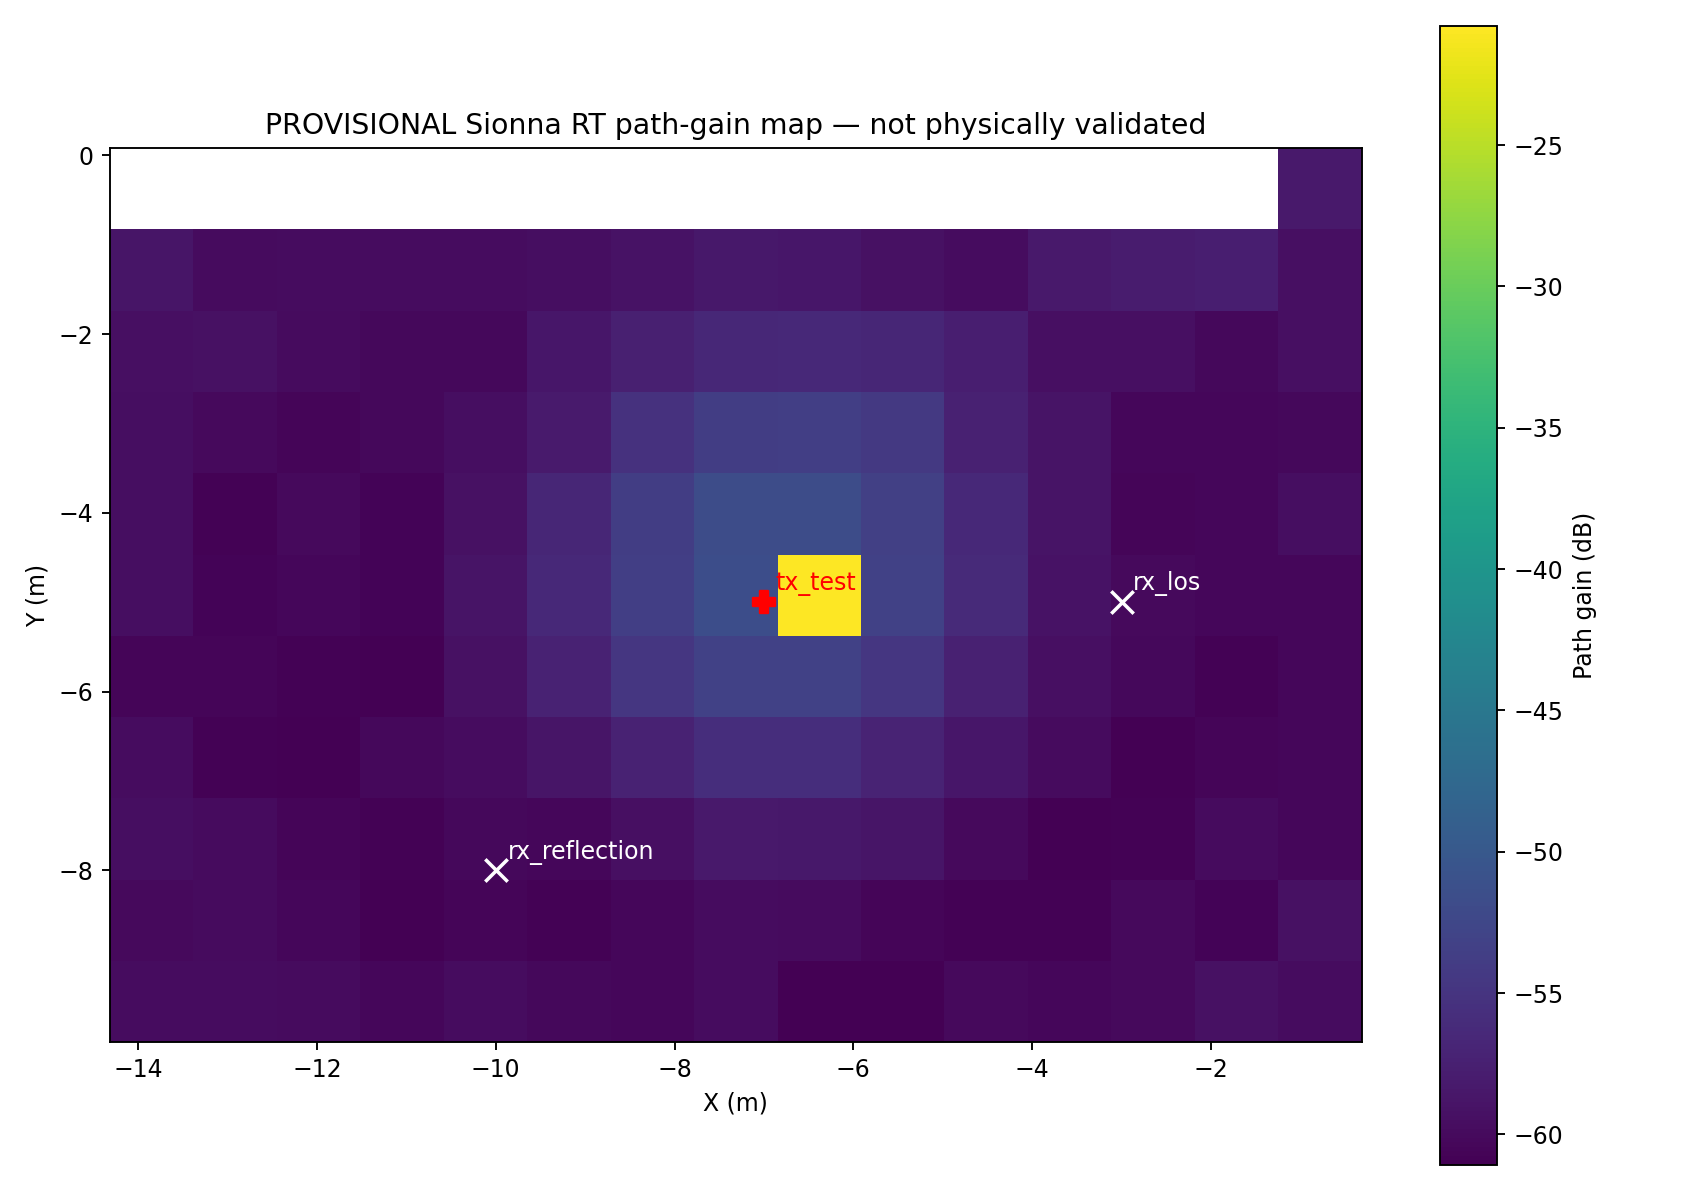
\includegraphics[width=\linewidth]{interim_figures/coverage_baseline.png}\par\small (a) 가상 벽 없음
  \end{minipage}\hfill
  \begin{minipage}{0.32\textwidth}\centering
    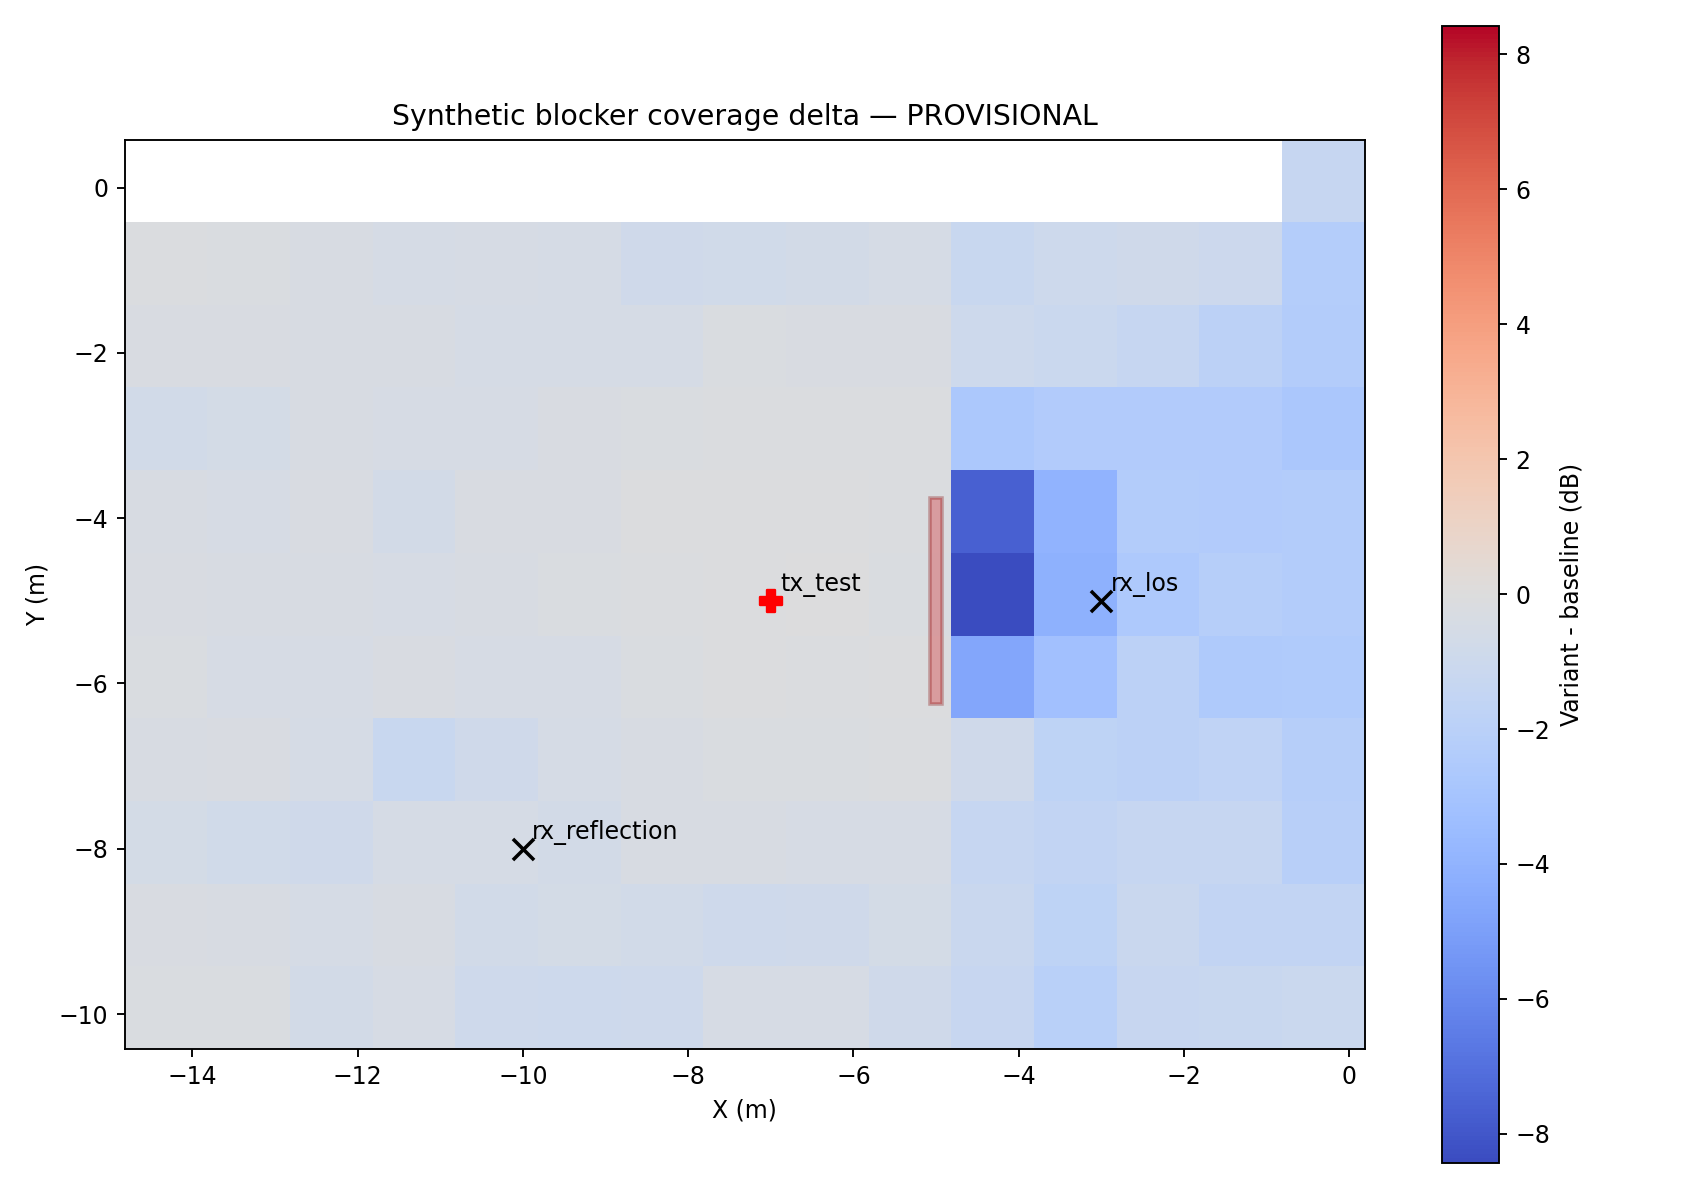
\includegraphics[width=\linewidth]{interim_figures/coverage_delta.png}\par\small (b) (c) $-$ (a)
  \end{minipage}\hfill
  \begin{minipage}{0.32\textwidth}\centering
    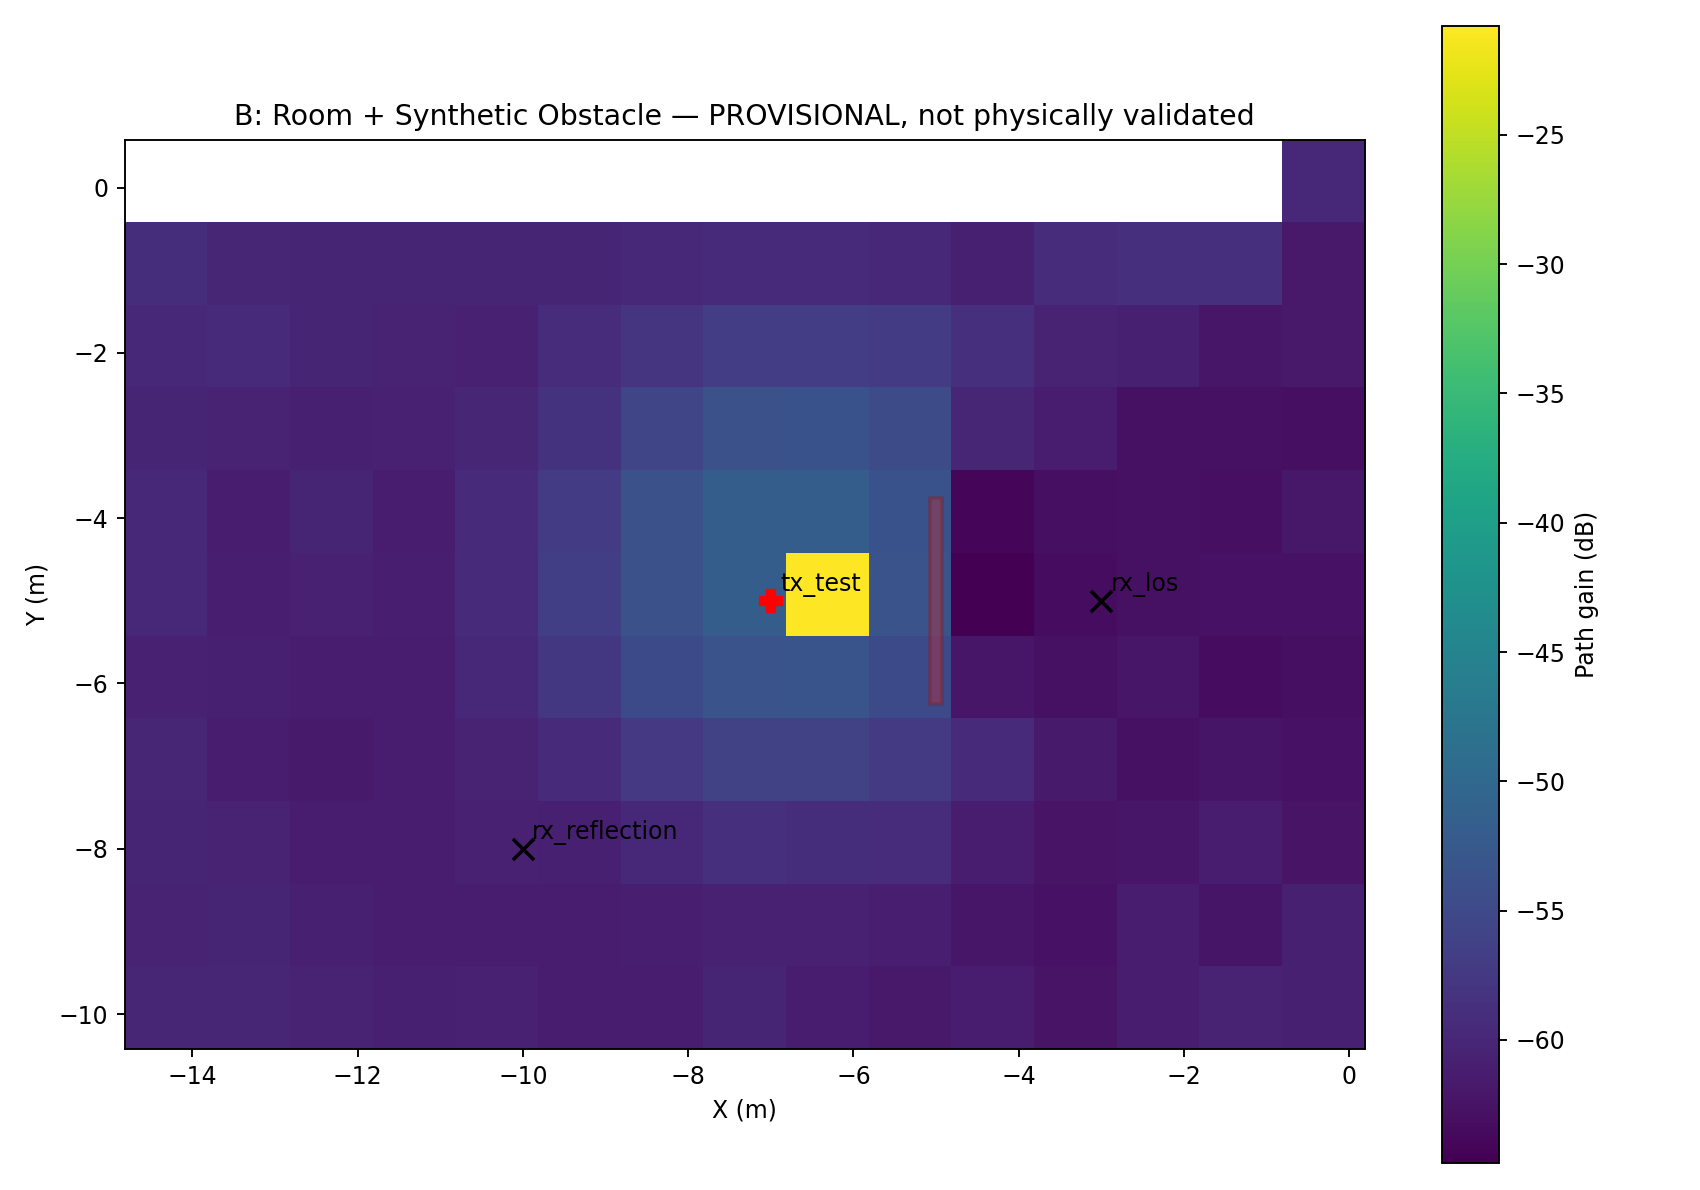
\includegraphics[width=\linewidth]{interim_figures/coverage_variant.png}\par\small (c) 가상 벽 있음
  \end{minipage}
  \caption{중간 단계 강의실 파일럿의 가상 벽 A/B 시험. 실제 구조와 재질을 검증한 결과가 아니라 구조물이 전파 계산에
  반영되는지 확인한 결과이다.}
  \label{fig:pilot-ab}
\end{figure}

\subsubsection{수집 경로와 백엔드 부하}

실물 게이트웨이 연동에서 다섯 소스의 표본 708건을 백엔드 내부 드롭 없이 저장하고 동기화 프레임 155개를 생성하였다.
수집 지연은 평균 146.67\,ms, p95 244\,ms, 최대 257\,ms였다. 모의 부하 시험에서는 노드 수를 2개에서 12개까지 늘리고
노드당 초당 10건을 발행하였다. 초당 약 120건까지 백엔드 수신 손실은 없었다(표~\ref{tab:pilot-load}). 다만 708건은 약
2분 20초 분량이므로 장시간 손실 추세를 보여 주지 못한다는 멘토 의견을 받았고, 이에 대한 보완은 \ref{sec:4.6}절과
\ref{sec:mentor}장에서 다룬다.

\begin{table}[htbp]
  \centering\small
  \caption{중간 단계 백엔드 모의 부하 시험 결과.}
  \label{tab:pilot-load}
  \begin{tabular}{@{}rrrrrr@{}}
    \toprule
    노드 수 & 발행/수신(건) & 손실률(\%) & 평균 지연(ms) & p95 지연(ms) & 프레임 생성 평균/최대(ms) \\
    \midrule
    2  & 398/398     & 0.00 & 68.8 & 125 & 1.7/3.9 \\
    4  & 796/796     & 0.00 & 74.0 & 130 & 1.8/3.9 \\
    8  & 1,592/1,592 & 0.00 & 81.2 & 128 & 1.8/3.9 \\
    12 & 2,388/2,388 & 0.00 & 86.0 & 144 & 1.8/3.9 \\
    \bottomrule
  \end{tabular}
\end{table}

\subsection{실험 설계}
\label{sec:4.1}

실험 공간은 중앙 코어를 둘러싼 링 형태의 복도로, 넓은 개방 복도와 좁은 복도가 코어를 사이에 두고 마주 본다. 이 배치는 코어 뒤편에 깊은 비가시선 영역을 만들면서도 링을 따라
우회하는 경로를 함께 제공하므로 결합 방식의 차이를 드러내기에 적합하다.

보정 지점은 가시선 2개와 비가시선 2개를 고루 포함하도록 배치하였다. 보정 집합이 한쪽 구간에만 있으면 반대 구간의 보정이 외삽이 되기 때문이다. 상세 조건은
표~\ref{tab:1}, 지점 배치는 그림~\ref{fig:3}에 제시한다.

\begin{table}[htbp]
  \centering\small
  \caption{실험 조건.}
  \label{tab:1}
  \begin{tabularx}{\textwidth}{@{}p{3.0cm} X@{}}
    \toprule
    항목 & 설정 \\
    \midrule
    송신기 & ipTIME N602SR 1대, 2.437\,GHz(채널 6), 높이 0.80\,m \\
    수신기 & ESP32 5대(고정 보정 4대 + 이동 시험 1대), 높이 0.45\,m \\
    시뮬레이션 설정 & 송신 전력 20\,dBm, 단일 등방성 안테나, 수직 편파, 콘크리트 프리셋(실측하지 않음) \\
    전파 현상 & 가시선, 정반사, 회절, 확산 산란 활성화; 벽 투과 제외; \texttt{max\_depth=12} \\
    보정 / 시험 지점 & 고정 4개(LoS 2개 + NLoS 2개) / 이동 10개(LoS 4개 + NLoS 6개) \\
    측정 절차 & test-10 $\rightarrow$ test-01의 단일 완주(관측치 10개); 지점당 20초 안정화 후 120초 기록 \\
    대표값 & 최근 유효 RSSI 표본의 이동평균에 대한 중앙값 + 실험 전 장치 편차 보정 \\
    \bottomrule
  \end{tabularx}
\end{table}

\begin{figure}[htbp]
  \centering
  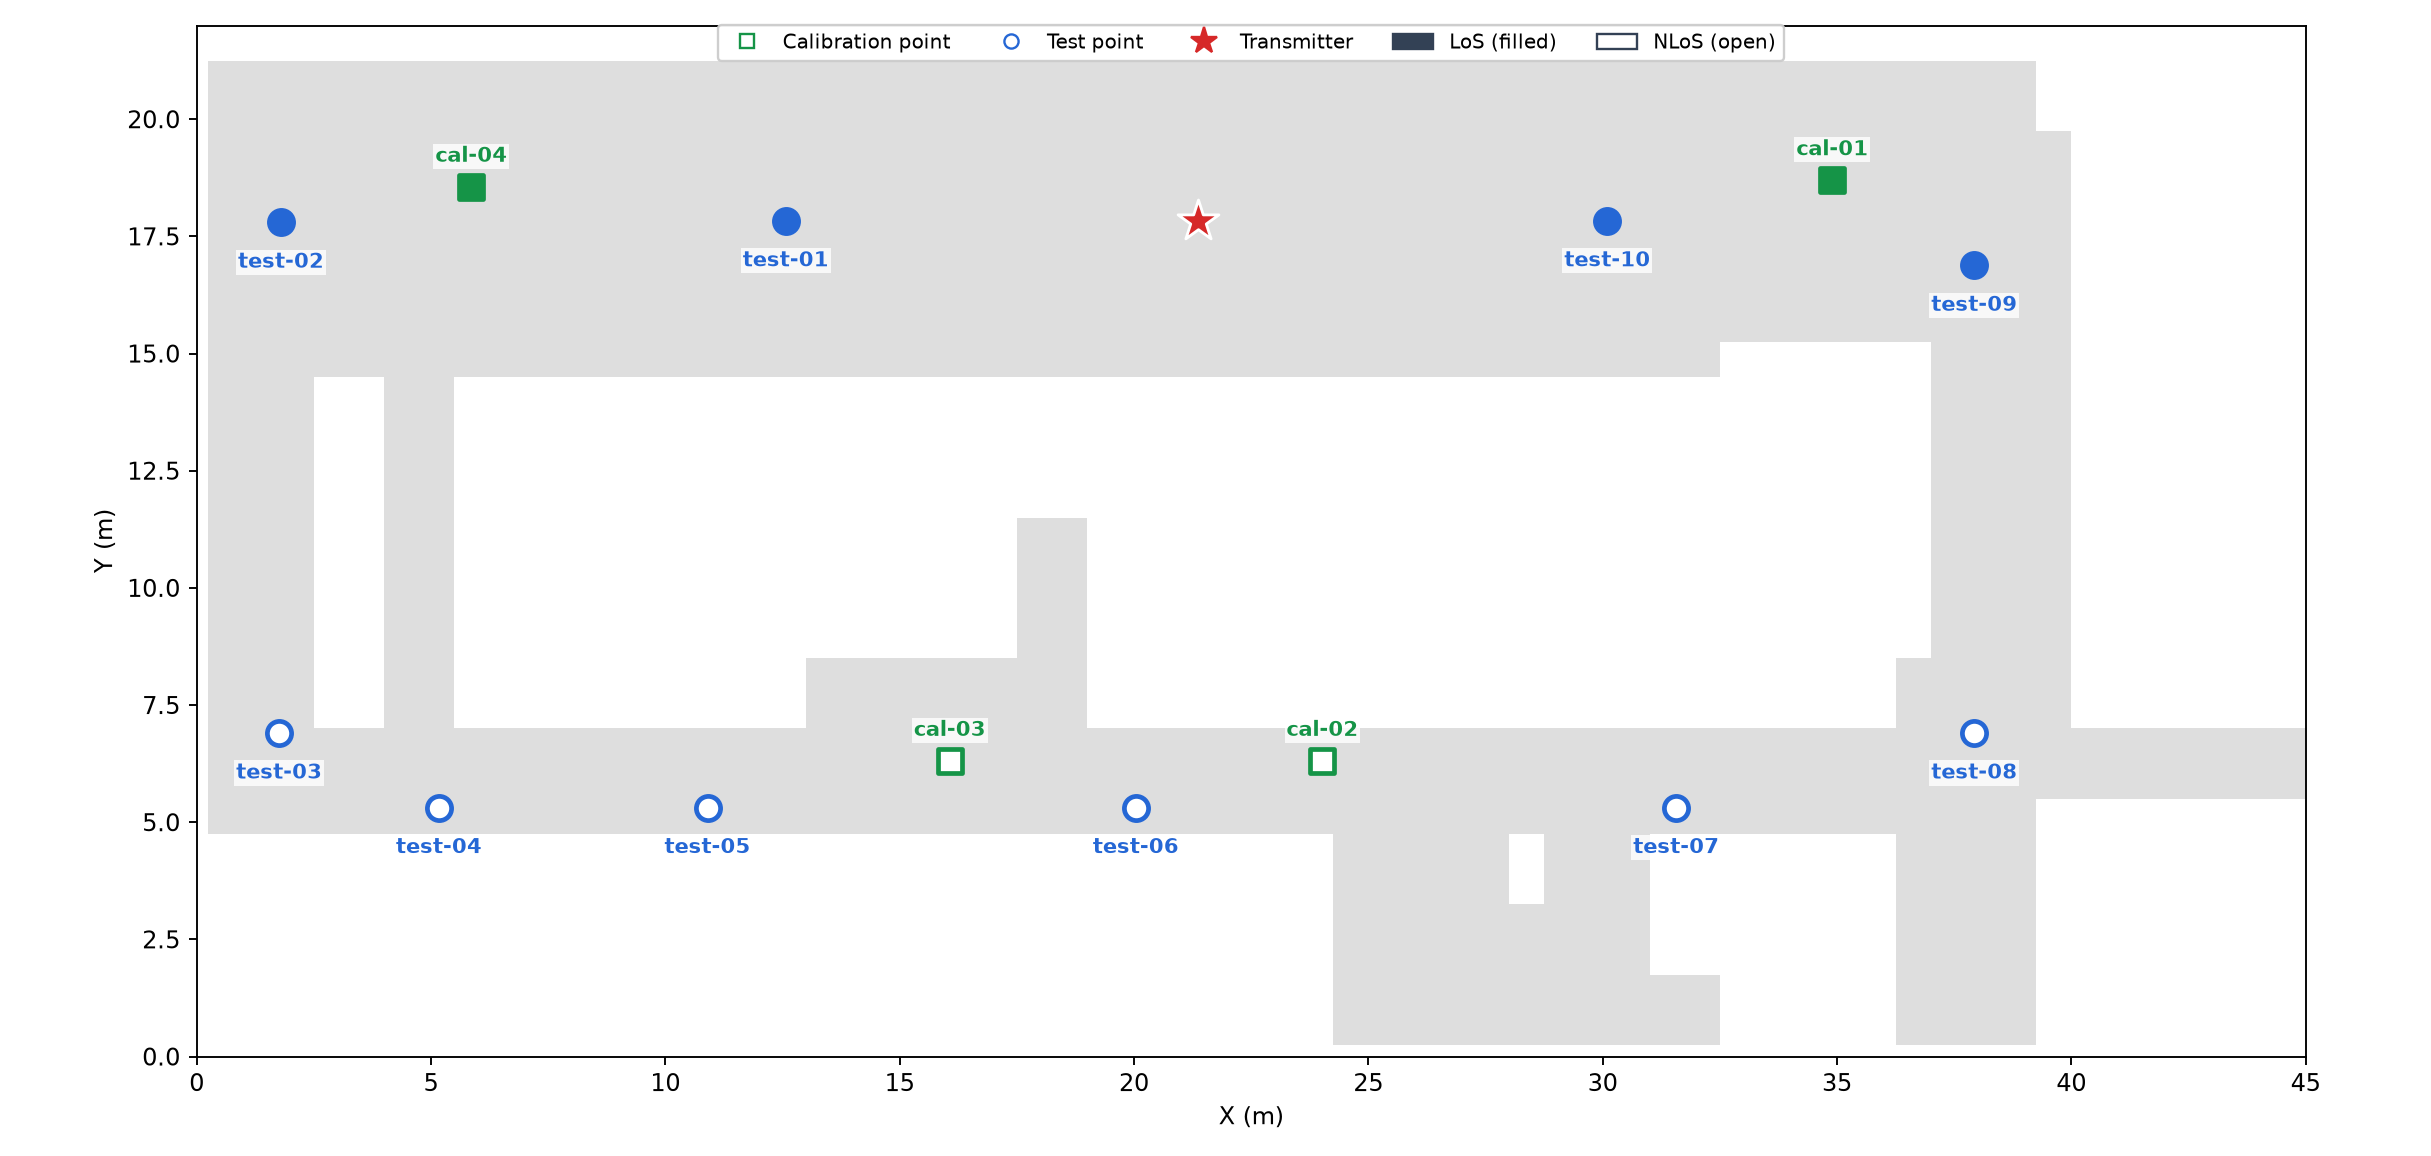
\includegraphics[width=1.0\textwidth]{paper/figure/fig3_v2.png}
  \caption{링 복도의 좌표계와 송신기, 고정 보정 지점 4개 및 시험 지점 10개의 배치.}
  \label{fig:3}
\end{figure}

\subsection{평가 지표}
\label{sec:4.2}

단일 측정 회차에서 각 시험 지점의 실측값과 예측값 사이의 MAE와 RMSE를 계산한다. 추가로 가시선 4개와 비가시선 6개 지점의 평균 편향과 방법별 MAE를 보고한다. 시험
지점의 실측값은 네 방법의 적합이나 보정에 사용하지 않고 평가에만 사용한다.

\subsection{방법별 예측 정확도}
\label{sec:4.3}

잔차 IDW는 비교한 네 방법 중 오차가 가장 낮았다. 단일 측정 회차에서 얻은 10개 시험 지점의 기술통계는 표~\ref{tab:2}와 같다. 잔차 IDW의 MAE는 이 표본에서
일반 IDW 대비 52.8\%, 원시 예측 대비 67.9\% 낮았다. 개별 지점 기준으로는 10개 중 7개에서 원시 예측보다 절대오차가 작았다. 보정 전 Sionna RT의 공간
예측 결과와 평가에 사용한 10개 지점은 그림~\ref{fig:4}와 같다.

\begin{table}[htbp]
  \centering\small
  \caption{단일 측정 회차의 시험 지점 10개에 대한 예측 오차.}
  \label{tab:2}
  \begin{tabular}{@{}lrr@{}}
    \toprule
    방법 & MAE (dB) & RMSE (dB) \\
    \midrule
    원시 예측 & 8.64 & 10.43 \\
    일반 IDW & 5.89 & 7.84 \\
    \textbf{잔차 IDW} & \textbf{2.78} & \textbf{4.13} \\
    전역 편향 보정 & 8.87 & 10.69 \\
    \bottomrule
  \end{tabular}
\end{table}

\begin{figure}[htbp]
  \centering
  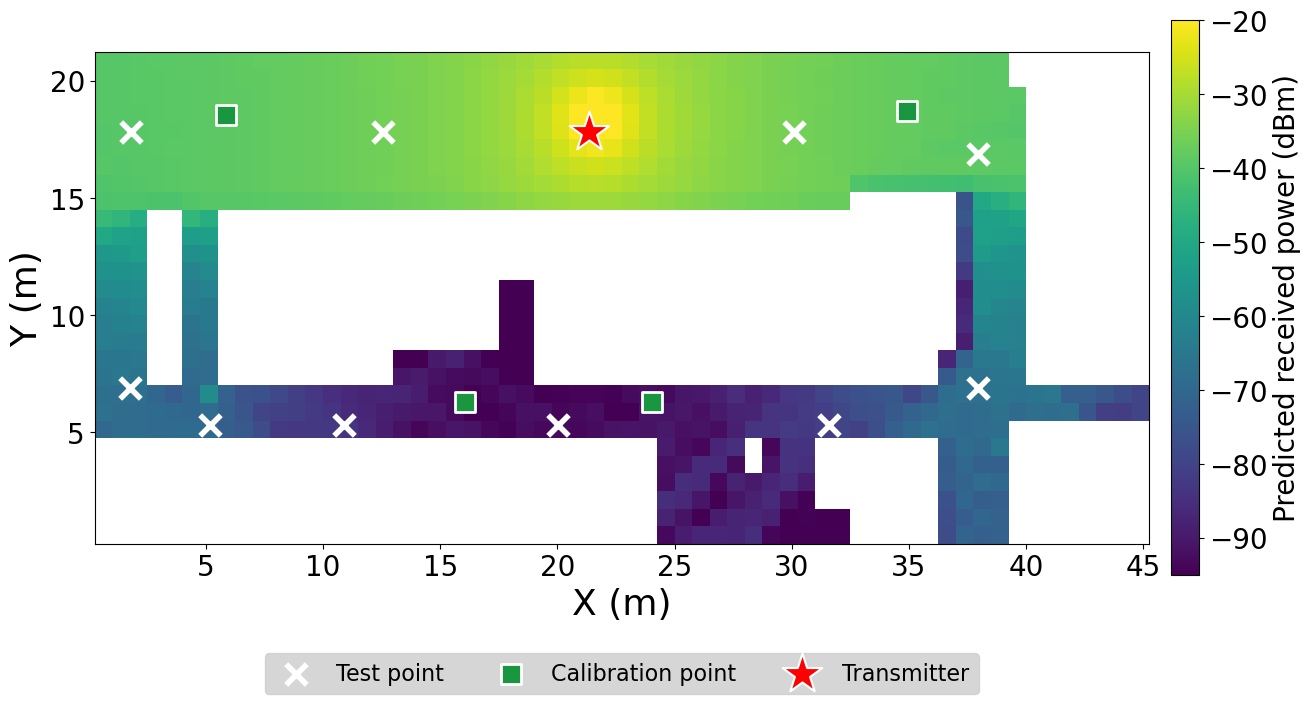
\includegraphics[width=1.0\textwidth]{paper/figure/fig4_v3.png}
  \caption{보정 전 Sionna RT의 예측 수신 전력 분포. 사각형은 보정 지점 4개, 십자 표시는 시험 지점 10개를 나타낸다.}
  \label{fig:4}
\end{figure}

\subsection{공간적 예측 편향 분석}
\label{sec:4.4}

LoS와 NLoS에서 평균 편향 방향이 반대로 나타났으며, 본 표본에서 전역 보정은 원시 예측의 오차를 줄이지 못했다(표~\ref{tab:2}, \ref{tab:3}). 여기서 Mean
Bias는 실측 RSSI에서 보정 전 Sionna RT 예측값을 뺀 값 $R-\hat{R}_S$의 평균으로 정의하며, 음수는 예측값이 실측값보다 큰 경우를 뜻한다. NLoS의 양의
편향은 코어 뒤편의 test-05와 test-06에서 각각 +12.6 dB와 +17.3 dB로 가장 컸다. 이는 벽 투과를 제외한 설정(\ref{sec:3.4}절)과 부합하지만,
본 데이터만으로 원인을 분리할 수는 없다.

\begin{table}[htbp]
  \centering\small
  \caption{관측치 10개의 구간별 예측 편향($R-\hat{R}_S$)과 방법별 MAE.}
  \label{tab:3}
  \begin{tabularx}{\textwidth}{@{}Xrrrrr@{}}
    \toprule
    구간 & $n$ & \shortstack{평균 편향\\(dB)} & \shortstack{원시 예측\\MAE (dB)} &
    \shortstack{일반 IDW\\MAE (dB)} & \shortstack{잔차 IDW\\MAE (dB)} \\
    \midrule
    가시선(LoS) & 4 & $-11.66$ & 11.66 & 8.31 & \textbf{1.59} \\
    비가시선(NLoS) & 6 & $+4.27$ & 6.63 & 4.28 & \textbf{3.57} \\
    \bottomrule
  \end{tabularx}
\end{table}

식~\eqref{eq:1}의 잔차를 공간적으로 보간한 결과는 그림~\ref{fig:5}과 같으며, 양수는 실측값이 예측값보다 큰 영역을 뜻한다.

\begin{figure}[htbp]
  \centering
  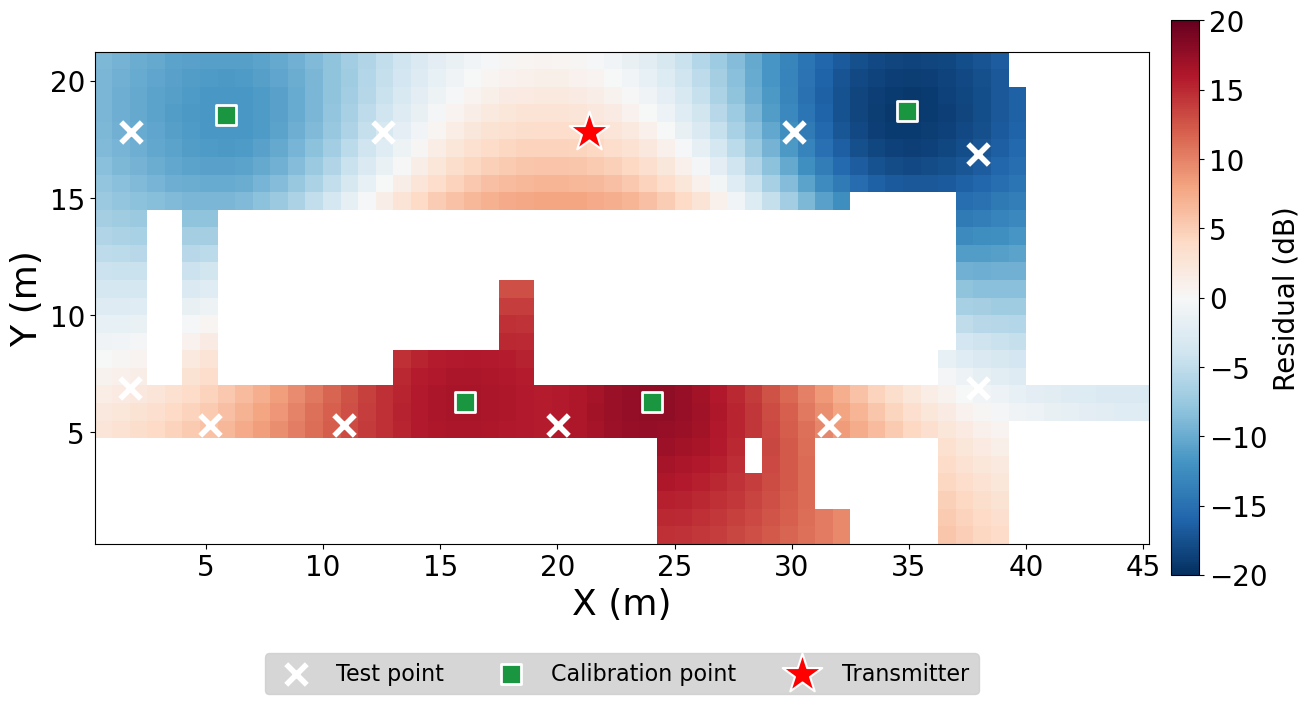
\includegraphics[width=1.0\textwidth]{paper/figure/fig5_v3.png}
  \caption{보정 지점의 잔차를 보간한 공간 잔차장. 표시에는 실행 전체의 보정값 평균을 사용하며, 정량 평가에는 시간창별 값을 사용한다.}
  \label{fig:5}
\end{figure}

잔차 IDW는 LoS와 NLoS 모두에서 일반 IDW보다 낮은 MAE를 보였으며, 개선 폭은 LoS에서 더 컸다. 다만 test-07에서는 인접 보정점의 잔차가 보간되면서 원시
예측보다 오차가 증가했다. 이는 잔차가 모든 위치에서 매끄럽게 변하지 않을 가능성을 시사한다. 또한 구조 정보는 예측항에만 반영되고 잔차 보간은 유클리드 거리를 사용하므로, 벽을
사이에 둔 보정점의 잔차가 실제 전파 경로와 무관하게 인접 영역으로 번질 수 있다. 코어 너머 NLoS 보정점 cal-02와 cal-03의 잔차는 각각 약 +17.8 dB와
+16.6 dB이며, 송신기와의 거리는 11.8 m와 12.7 m로 LoS 보정점(13.6\,m, 15.5\,m)보다 가깝다. 이 때문에 그림~\ref{fig:5}에서는 송신기
반경 3\,m 이내의 LoS 영역에도 평균 약 +3\,dB, 최대 약 +8 dB의 양의 잔차가 보간되었다. 잔차 IDW로 생성한 복도 RF 지도는 그림~\ref{fig:6}과
같다.

\begin{figure}[htbp]
  \centering
  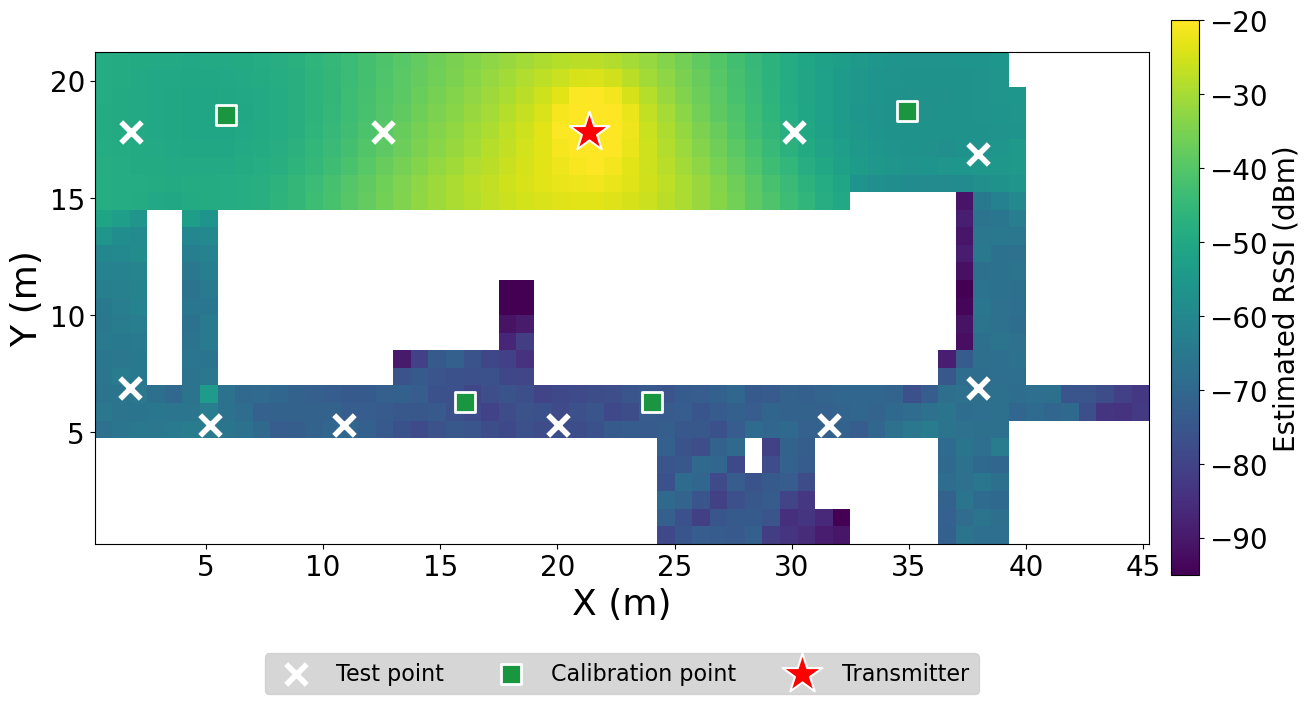
\includegraphics[width=1.0\textwidth]{paper/figure/fig6_v3.png}
  \caption{잔차 IDW로 생성한 복도 RF 지도. 표시에는 실행 전체의 보정값 평균을 사용한다.}
  \label{fig:6}
\end{figure}

\begin{samepage}
재구성 장면 위에 RF 볼륨을 중첩한 PC 렌더러 화면은 그림~\ref{fig:7}와 같다. (a)는 송신기가 있는 넓은 LoS 복도의 잔차 IDW 결과이고, (b)와 (c)는
코어 뒤편 NLoS 복도를 같은 시점에서 원시 예측과 잔차 IDW로 전환한 결과이다. 원시 예측에서 낮게 표시된 NLoS 복도의 수신 전력이 잔차 보정 후 높게 표시되는 것을
확인할 수 있다.
\end{samepage}

\begin{figure}[htbp]
  \centering
  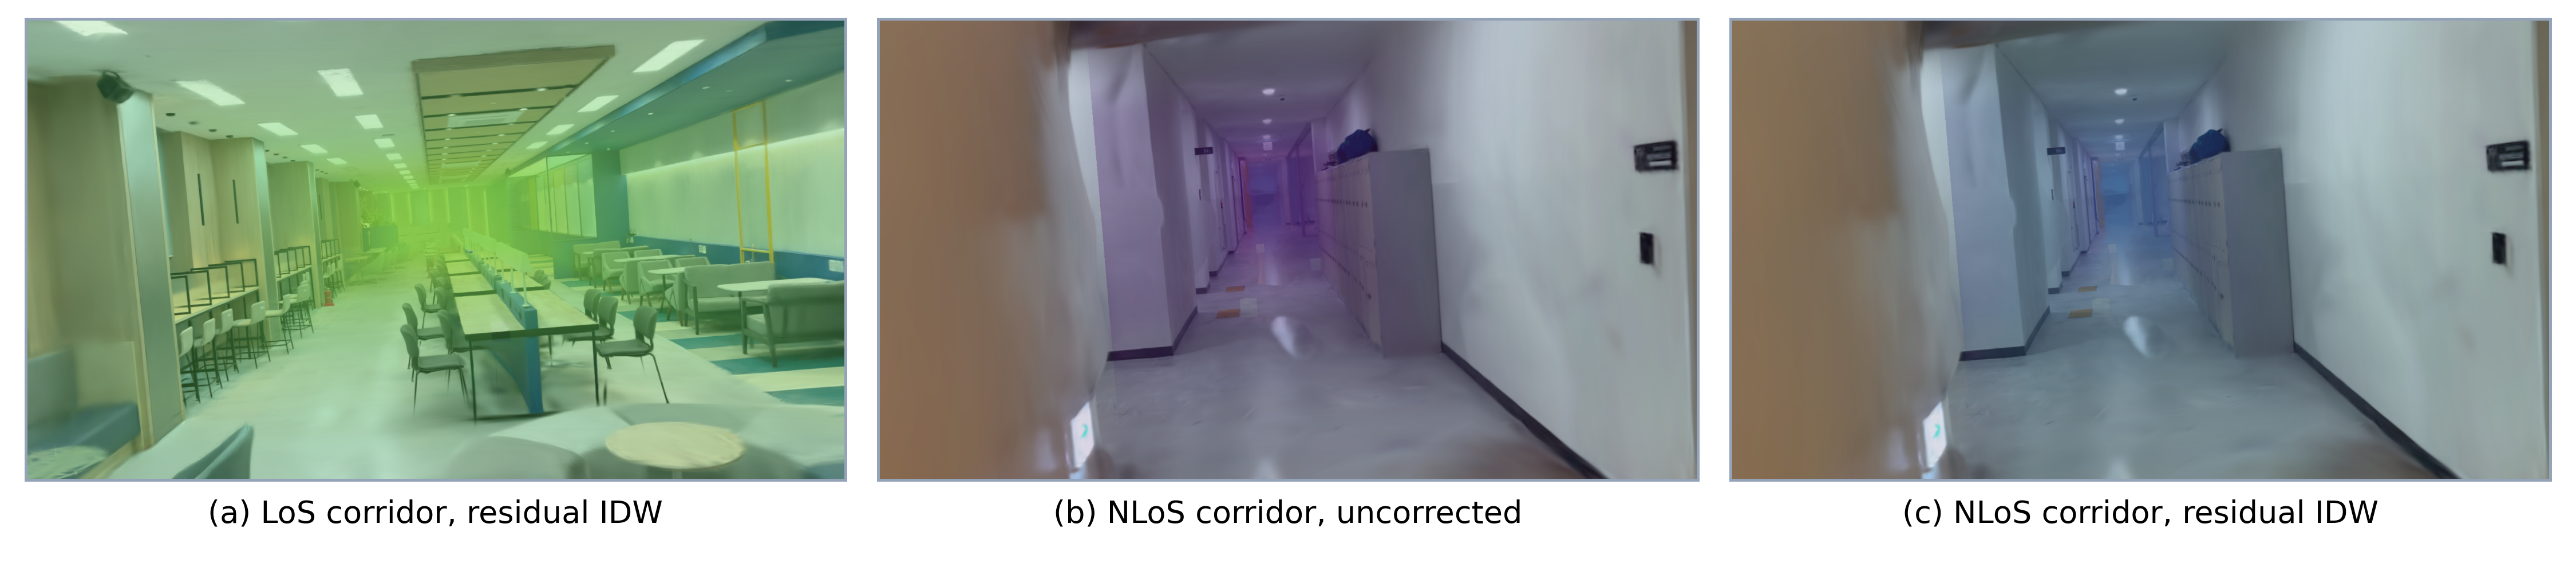
\includegraphics[width=1.0\textwidth]{paper/figure/fig7_v3.png}
  \caption{재구성 장면 위에 RF 볼륨을 중첩한 PC 렌더러 화면. (a) 넓은 가시선 복도의 잔차 IDW 결과. (b) 코어 뒤편 비가시선 복도의 원시 예측과 (c) 같은 시점의 잔차 IDW 결과.}
  \label{fig:7}
\end{figure}

\begin{samepage}
\subsection{시스템 기능 검증}
\label{sec:4.5}

구현한 시각화 시스템의 기능은 실제 ESP32-S3 핸드헬드와 렌더러를 연결한 상태에서 확인하였다. 렌더링
영상이 핸드헬드 디스플레이에 출력되었고, 실제 장착 상태의 IMU 자세 변화에 따라 카메라가 회전하였다.
또한 텔레포트 버튼을 사용해 조준한 이동 후보 위치로 이동할 수 있었으며, 높이 순환 버튼을 누를 때 표시되는 RF
볼륨의 높이가 순차적으로 전환되었다. 검증에 사용한 핸드헬드 장치는 그림~\ref{fig:8}과 같다.

영상, IMU와 버튼을 함께 활성화한 300초 이상의 운용 구간에서 화면 정지나 기능 중단은 관찰되지 않았다.
이는 RF 정확도 평가와 별도로 수행한 정성적 기능 확인이며, 지속 프레임률, 종단 지연과 전송 손실률의
정량 평가는 향후 과제로 남는다.

기존 호스트 시험 기록에서는 STM32 파서와 JSON 생성, Python 브리지, RFJF 헤더 파서와 RFHC
직렬화의 동작 및 RGB565에서 RGB666으로의 패킹 등가성을 확인하였다. 이는 실기기 처리율과 종단 지연
평가와 구분된다.
\end{samepage}

\begin{figure}[htbp]
  \centering
  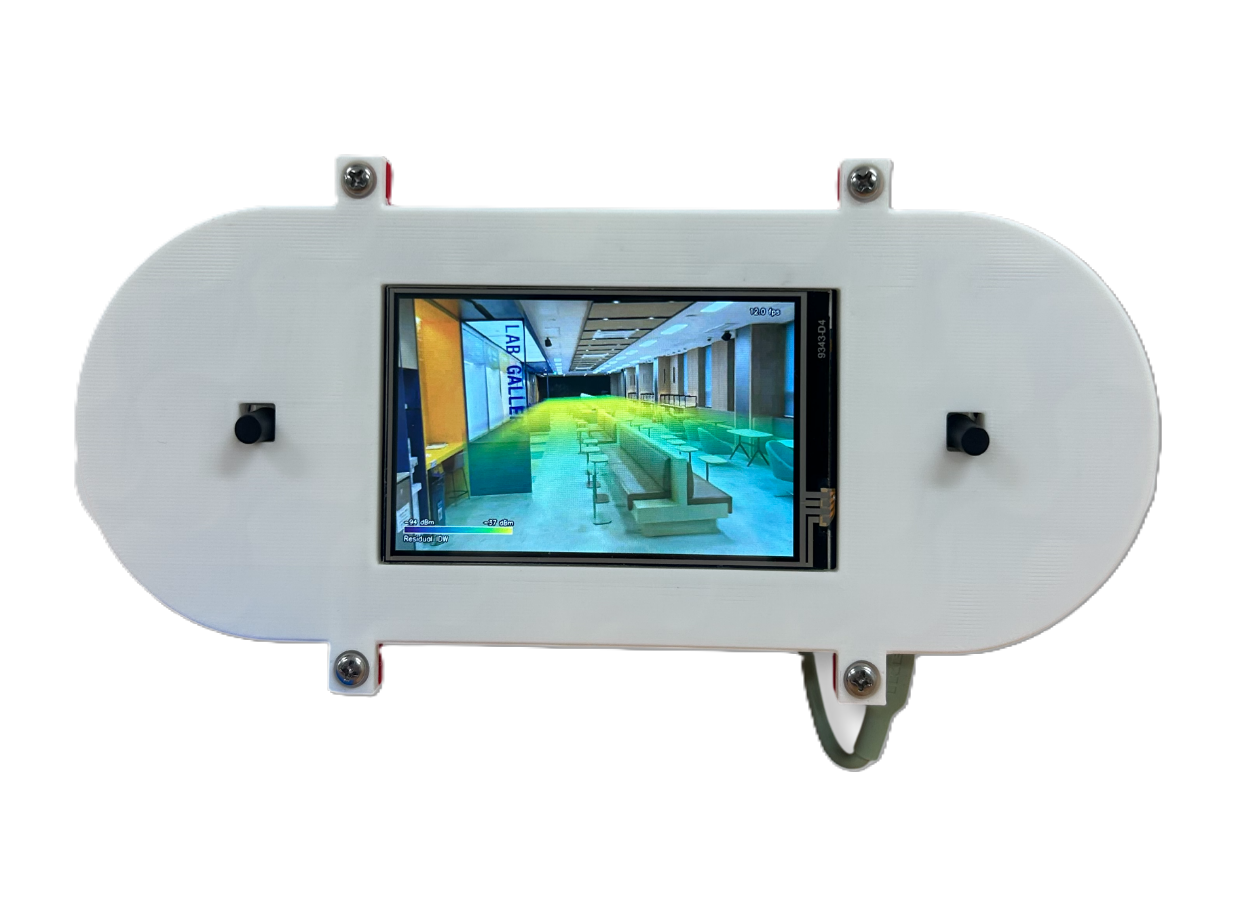
\includegraphics[width=0.72\textwidth]{paper/figure/fig8_v2.png}
  \caption{시스템 기능 검증에 사용한 ESP32-S3 핸드헬드 시제품.}
  \label{fig:8}
\end{figure}

\subsection{계측 데이터 품질과 연속 운용}
\label{sec:4.6}

중간 단계의 708건은 약 2분 20초 분량이어서 장시간 손실 추세를 확인할 수 없었다. 이를 보완하기 위해 최종 측정 회차
(2026년 8월 21일 21:38 $\sim$ 22:23, 2,725\,s)의 원시 자료로 노드별 순번 누락, 수신 간격과 시각 차이를 분석하였다.
고정 보정 노드 네 대는 회차 전체를 끊지 않고 기록하므로 약 45분 연속 운용 자료가 된다. 원격 노드는 약 1초마다 순번을
하나씩 올려 전송하므로, 수신한 순번의 최소 $\sim$ 최대 범위를 기대 표본 수로 보았다. 결과는 표~\ref{tab:quality}와 같다.

\begin{table}[htbp]
  \centering\small
  \caption{45분 연속 측정 회차의 고정 보정 노드별 수집 품질. 시각 차이는 서버 수신 시각에서 노드 측정 시각을 뺀 값이며
  노드와 서버의 시계 오프셋을 포함한다.}
  \label{tab:quality}
  \begin{tabular}{@{}llrrrrr@{}}
    \toprule
    장치 & 역할 & \shortstack{수신/기대\\(건)} & \shortstack{순번 누락\\(\%)} & \shortstack{최대 수신\\간격(s)} &
    \shortstack{시각 차이\\중앙값(ms)} & \shortstack{시각 차이\\p95(ms)} \\
    \midrule
    gw-01   & cal-04 & 2,678/2,693 & 0.56  & 3.5 & 329 & 464 \\
    node-01 & cal-01 & 2,487/2,717 & 8.47  & 4.4 & 450 & 617 \\
    node-03 & cal-02 & 1,840/2,720 & 32.35 & 9.0 & 481 & 714 \\
    node-04 & cal-03 & 2,062/2,718 & 24.14 & 9.1 & 425 & 616 \\
    \bottomrule
  \end{tabular}
\end{table}

모든 노드에서 중복과 역순 도착은 없었다. 반면 순번 누락률은 게이트웨이 자체 측정(0.56\,\%)과 원격 노드(8.47 $\sim$
32.35\,\%) 사이에 큰 차이가 있었다. 누락은 코어 뒤편 비가시선의 cal-02(node-03)와 cal-03(node-04)에서 컸다. 이는
ESP-NOW 무선 구간의 손실과 관련이 있을 가능성이 있으나, 무선, UART, STM32의 장치별 최신 상태 갱신 중 어느 구간에서
표본이 빠졌는지는 분리하지 않았다. 원격 노드의 최대 수신 간격은 9.1\,s로, 수 분 이상 이어진 연결 단절은 없었다.

누락이 있어도 각 시험 구간의 120\,s 기록창에는 고정 노드마다 67 $\sim$ 119개, 이동 노드는 68 $\sim$ 119개의 표본이
남았다. 대표값은 이 표본의 중앙값이므로 분석에 필요한 표본 수는 확보되었다. 그러나 2분대 시험에서는 드러나지 않던
노드별 손실 차이가 45분 자료에서 확인되었다. 따라서 장시간 운용에는 원격 노드의 재전송이나 배치 조정이 필요하다.
노드 측정 시각과 서버 수신 시각의 차이는 p95 기준 464 $\sim$ 714\,ms였다. 이 값은 시계 오프셋을 포함하므로 순수
전송 지연으로 해석하지 않는다. 한편 실시간 경로의 유예 구간 기본값 300\,ms는 중간 단계의 p95 244\,ms를 기준으로
정한 것이므로, 이 분포를 반영하여 다시 정할 필요가 있다. 이번 분석 자료에는 재연결 시간과 ESP32 heap 잔량이 포함되어
있지 않다.

\section{산학협력 멘토 의견 반영}
\label{sec:mentor}

중간보고서에 대해 2026년 8월 1일 망고부스트코리아 서준오 연구원의 서면 자문을 받았다. 자문은 Message Queue와
WebSocket으로 구성한 준실시간 처리 구조, PGSR 메시의 구멍과 노이즈를 인정하고 닫힌 Proxy Mesh 경로를 추가한 판단을
긍정적으로 평가하였다. 보완이 필요한 사항으로는 노드 측정 시각, 시간창 기준과 장시간 시험의 세 가지를 지적하였다.
각 의견에 대한 대응은 표~\ref{tab:mentor}와 같다.

{\small
\renewcommand{\arraystretch}{1.2}
\begin{longtable}{@{}>{\raggedright\arraybackslash}p{3.6cm}
  >{\raggedright\arraybackslash}p{5.6cm}
  >{\raggedright\arraybackslash}p{5.7cm}@{}}
\caption{산학협력 멘토 의견과 대응.}\label{tab:mentor}\\
\toprule
멘토 의견 & 대응 및 반영 내용 & 확인 결과와 남은 과제 \\
\midrule
\endfirsthead
\toprule
멘토 의견 & 대응 및 반영 내용 & 확인 결과와 남은 과제 \\
\midrule
\endhead
\bottomrule
\endfoot
\textbf{① 노드 timestamp 저장.} 게이트웨이 시각이 아닌 각 노드의 측정 시각을 센서 값과 함께
저장해야 한다. &
자문이 검토한 중간 단계 실시간 경로는 게이트웨이 시각만 사용하였다. 중간보고 이후 재설계한 측정 경로는 측정 시각이
포함된 ESP-NOW 버전 2 패킷을 사용하고, 노드와 게이트웨이의 시각을 SNTP로 맞춘다. 동기화 전 표본은 시각 무효
플래그로 구분한다. 백엔드는 노드 측정 시각과 서버 수신 시각을 별도 열로 저장하고, 분석용 원본 자료와 실시간 프레임에도
두 시각을 함께 담는다(\ref{sec:3.5}, \ref{sec:network}절). &
최종 회차의 원시 자료 10,351건 모두 두 시각을 함께 가진다. 두 시각의 차이로 노드별 지연 분포를 산출하였다
(표~\ref{tab:quality}). 노드 간 시계 오프셋과 순수 전송 지연은 분리하지 않았다. \\
\midrule
\textbf{② 측정 시각 기준 시간창과 유예 구간.} p95 244\,ms가 200\,ms 창을 넘으므로 도착
시각 기준 묶음이 측정 시점과 어긋난다. &
실시간 경로의 시간창을 노드 측정 시각 기준으로 바꾸고, 300\,ms의 늦은 도착 유예 구간을 두었다. 확정은 측정 시각
워터마크로 판단하고, 입력이 멈추면 서버 시계로 창을 닫는다. 유예 뒤 도착한 표본은 별도로 집계한다
(8월 11일 반영). 정지 측정은 120\,s 기록창과 같은 시간창의 보정 자료를 사용한다(\ref{sec:3.6}절). &
시간창 단위 시험 7건(측정 시각 배정, 유예 내 포함, 유예 후 제외, 워터마크 확정, 입력 정지 시 확정 등)이 통과하였다.
최종 정확도 실험은 정지 측정 경로를 사용하였으므로 실시간 시간창은 실험 결과에 영향을 주지 않는다. 45분 자료의
시각 차이 p95(464 $\sim$ 714\,ms)를 반영하여 유예 구간을 다시 정해야 한다. \\
\midrule
\textbf{③ 30분 이상 연속 시험.} 708건은 약 2분 20초 분량이므로 순번 손실, 재연결 시간과
heap 잔량을 장시간 기록해야 한다. &
백엔드의 지표 API를 주기적으로 조회하여 순번 손실 누계, MQTT 연결 해제 횟수, 수집 지연과 노드 온라인 수를 시계열로
남기는 장시간 모니터링 도구를 추가하였다(단위 시험 4건 통과). 또한 최종 측정은 고정 노드가 끊김 없이 기록되는 45분
연속 회차로 수행하였다. &
45분 자료에서 노드별 순번 누락률 0.56 $\sim$ 32.35\,\%와 최대 9.1\,s의 수신 간격을 확인하였다(\ref{sec:4.6}절).
2분대 시험에서 보이지 않던 노드 간 손실 차이이다. 재연결 시간과 ESP32 heap 잔량의 장시간 기록은 수행하지 못해 향후
과제로 남긴다. \\
\end{longtable}
}

\section{결론 및 향후 연구 방향}
\label{sec:5}

\subsection{연구 결과 요약}

본 보고서는 사진 기반 3DGS 장면, Sionna RT와 ESP32 RSSI 측정을 결합하고, 시뮬레이션과 실측의 잔차를 공간적으로 보간하는 방법을 제안하였다. 단일 링 복도의
10개 시험 지점을 모두 포함하는 1회 측정에서 잔차 IDW는 비교한 네 방법 중 가장 낮은 MAE 2.78 dB를 보였으며, 일반 IDW 대비 52.8\%, 원시 예측 대비
67.9\% 낮았다. 또한 LoS와 NLoS의 편향 방향이 달라 모든 위치에 같은 보정값을 적용하는 방식에는 한계가 있음을 확인하였다.

시스템 측면에서는 다섯 ESP32 계측부, MQTT 백엔드, 3DGS 렌더러와 ESP32-S3 핸드헬드를 하나의 좌표계와 공통 규약으로
연결하였다. 착수보고서의 과제 목표별 달성 정도는 표~\ref{tab:goals}와 같다.

\begin{table}[htbp]
  \centering\small
  \caption{착수 단계 과제 목표 대비 최종 결과.}
  \label{tab:goals}
  \renewcommand{\arraystretch}{1.2}
  \begin{tabularx}{\textwidth}{@{}>{\raggedright\arraybackslash}p{3.6cm}
    >{\raggedright\arraybackslash}X >{\centering\arraybackslash}p{1.5cm}@{}}
    \toprule
    과제 목표 & 최종 결과 & 달성도 \\
    \midrule
    다중 노드 RSSI 계측 & 고정 보정 4대와 이동 시험 1대로 링 복도 10개 시험 지점을 측정, 45분 연속 운용 자료 확보 & 달성 \\
    수집, 검증, 시간 정합 파이프라인 & Mosquitto 수집, 입력 검증, 두 시각 저장, 측정 시각 기준 시간창, Run/TestSegment, 내보내기와 품질 검사 & 달성 \\
    3DGS 장면 재구성 & 강의실(파일럿)과 3층 링 복도의 PGSR 장면, 닫힌 프록시와 미터 좌표계 & 달성 \\
    RF 신호장 추정과 3차원 시각화 & Sionna RT와 잔차 IDW(MAE 2.78\,dB), 여섯 높이 RF 볼륨, 렌더러 합성과 핸드헬드 탐색 & 달성(방법 변경) \\
    성능 지표 평가 & MAE/RMSE, 백엔드 부하와 지연, 노드별 순번 누락 분석. 영상 경로의 지속 프레임률과 종단 지연은 미정량 & 부분 달성 \\
    \bottomrule
  \end{tabularx}
\end{table}

\subsection{한계 및 향후 연구}

다만 본 평가는 한 건물의 한 개 층, 단일 송신기와 채널, 네 개 보정 지점 및 1회 측정에 한정된 기술통계이며, 반복 측정에 따른 변동은 정량화하지 못했다. 시뮬레이션에는
명목값과 이상화된 안테나/재질 모델을 사용하였다. 본 평가는 RSSI 기반 수신 세기 비교에 한정되며, 정밀 채널 특성은 측정하지 않았다. 잔차의 개별 물리적 원인도 분리하지
않았으며, 실험 후 장치 편차를 다시 측정하지 않아 실험 중 감도 변화를 확인하지 못했다.

잔차 IDW는 test-07처럼 원시 예측이 정확한 위치의 오차를 키울 수 있으며, 벽을 사이에 둔 지점 사이로 잔차가 번질 수 있다. 다른 높이에 적용한 RF 볼륨은 정성적
시각화에 한정된다. 향후에는 다양한 공간, 시간, 높이에서 보정 지점 배치와 NLoS 잔차를 평가하고, 벽을 가로지르는 연결을 제한하는 영역 분리 또는 장애물 인지 거리 보간과
재질/투과손실 측정을 검증할 예정이다. 시각화 시스템의 지속 표시율, 종단 지연과 전송 손실률도 정량화할 예정이다.
계측부는 원격 노드의 순번 누락을 줄이기 위한 재전송과 배치 조정을 검토한다. 멘토 의견에 따라 재연결 시간과 ESP32 heap
잔량을 포함한 1시간 이상 연속 시험을 수행하고, 실시간 시간창의 유예 구간을 측정 분포에 맞게 다시 정할 계획이다.

\clearpage
\section{구성원별 역할 및 개발 일정}
\label{sec:roles}

\subsection{구성원별 역할}

구성원별 역할은 표~\ref{tab:roles}와 같다.

\begin{table}[htbp]
  \centering\small
  \caption{팀원별 역할 분담.}
  \label{tab:roles}
  \renewcommand{\arraystretch}{1.2}
  \begin{tabularx}{\textwidth}{@{}p{2.1cm} p{1.3cm} >{\raggedright\arraybackslash}X@{}}
    \toprule
    학번 & 성명 & 담당 역할 \\
    \midrule
    202355708 & 이승우 &
    \textbullet\ PGSR을 이용한 실내 공간의 3D Gaussian Splatting 장면 재구성 및 표면 메시 추출\newline
    \textbullet\ 전파 계산에 적합한 닫힌 공간 모델 생성\newline
    \textbullet\ Sionna RT 기반 전파 경로 및 신호 분포 계산\newline
    \textbullet\ SIBR Viewer 3D RF 볼륨 시각화 및 영상 송신, 핸드헬드 시점 제어 연동 \\
    \midrule
    202355701 & 강주호 &
    \textbullet\ Mosquitto MQTT 브로커 구성 및 다중 RSSI 노드와 게이트웨이 데이터 수집 구조 구축\newline
    \textbullet\ 수신 데이터 검증 및 필터링과 시간창 기반 동기화를 통한 지점별 측정 프레임 생성\newline
    \textbullet\ 노드 상태, 손실, 지연시간 모니터링 및 실시간 대시보드 구현\newline
    \textbullet\ WebSocket, REST API를 통한 그래픽스 데이터 전달과 임베디드/그래픽스 간 메시지 규격 관리 \\
    \midrule
    202355707 & 이나영 &
    \textbullet\ ESP32 기반 다중 RSSI 측정 노드와 ESP-NOW 게이트웨이 구조 설계 및 펌웨어 구현\newline
    \textbullet\ RSSI 측정값의 이동평균 처리, 패킷 오류 검사 및 노드별 수신, 중복, 누락 상태 관리\newline
    \textbullet\ STM32 UART 수신, 전처리, JSON 생성과 시리얼--MQTT 브리지를 통한 서버 전송 경로 구축\newline
    \textbullet\ 다중 실물 노드 및 장시간 안정성 검증과 핸드헬드 IMU, 버튼, LCD 영상 출력 기능 구현 \\
    \midrule
    공통 & 전원 &
    \textbullet\ 파트 간 인터페이스(RSSI 자료 형식, RFJF 영상 프레임, RFHC 제어 패킷, 분석용 내보내기) 합의\newline
    \textbullet\ 3층 복도 실측, 통합 시험과 시연 준비\newline
    \textbullet\ 착수, 중간, 최종보고서와 학술 원고 작성 \\
    \bottomrule
  \end{tabularx}
\end{table}

\FloatBarrier
\subsection{계획 대비 추진 실적}

착수보고서는 5월부터 9월까지 세 파트가 병렬로 개발하고 8월 이후 통합과 성능 분석을 수행하는 일정을 세웠다.
중간보고서는 최종 통합의 선행조건을 기준으로 이 일정을 표~\ref{tab:plan}의 왼쪽 두 열과 같이 갱신하였다.
각 항목의 실제 추진 결과는 오른쪽 열과 같다.

{\small
\renewcommand{\arraystretch}{1.2}
\begin{longtable}{@{}>{\raggedright\arraybackslash}p{1.6cm}
  >{\raggedright\arraybackslash}p{4.6cm}
  >{\raggedright\arraybackslash}p{7.0cm}
  >{\centering\arraybackslash}p{1.3cm}@{}}
\caption{중간보고서의 갱신 계획 대비 추진 실적.}\label{tab:plan}\\
\toprule
계획 시기 & 계획 작업 & 실제 추진 결과 & 상태 \\
\midrule
\endfirsthead
\toprule
계획 시기 & 계획 작업 & 실제 추진 결과 & 상태 \\
\midrule
\endhead
\bottomrule
\endfoot
7월 하순 & 메시지 형식 동결, 3대 이상 실물 노드 30분 이상 시험 & 다섯 장치로 45분 연속 측정. 대상 AP의 BSSID와 채널은 실험 전 고정·기록 & 완료 \\
7월 하순 & 강의실 치수 실측, 노드 설치 좌표 기록 & 대상 공간을 3층 링 복도로 변경. 층고 기반 배율, 도면 정합과 표식 좌표 확정 & 변경 \\
7월 하순 & 재연결, 링 버퍼, Watchdog, 상태 지표 & STM32 링 버퍼, DMA 시간 초과 시 재부팅, 구간 중단 표시와 장시간 모니터링 도구 구현. 자동 재연결 실동작은 미검증 & 부분 \\
8월 초 & SIBR에서 Gaussian 로드와 히트맵 평면 표시 & 평면 대신 여섯 높이 RF 볼륨을 렌더러에 합성 & 변경 \\
8월 초 & 실측 RSSI와 Sionna 결과 비교, 보정 기준 결정 & 복도 실측과 네 방법 비교로 잔차 IDW 채택 & 완료 \\
8월 중순 & 메시 깊이 기반 히트맵 가림 & 프록시 메시 깊이 기반 가림 구현 & 완료 \\
8월 중순 & IMU 쿼터니언 수신, 버튼식 위치 갱신 & IMU 자세 연동. 버튼 기능을 텔레포트와 높이 순환으로 변경하고 실물 종단 확인 & 변경 \\
8월 하순 & JPEG 인코딩, TCP 전송, LCD 표시 & RFJF 규격으로 실기기 종단 영상 출력과 LCD 병목 최적화. 지속 프레임률은 미정량 & 부분 \\
9월 & 전체 통합과 종단 성능 측정 & 영상, IMU, 버튼을 함께 연결한 300초 이상 운용에서 기능 지속 확인. 종단 지연은 미정량 & 부분 \\
\end{longtable}
}

\subsection{월별 추진 타임라인}

착수보고서, 중간보고서와
\href{https://github.com/2026-PNU-CSE-GRAD-RFVisualizer/Embedded/commits}{임베디드},
\href{https://github.com/2026-PNU-CSE-GRAD-RFVisualizer/RFVisualizer/commits}{그래픽스},
\href{https://github.com/2026-PNU-CSE-GRAD-RFVisualizer/Network-Backend/commits}{네트워크 초기},
\href{https://github.com/2026-PNU-CSE-GRAD-RFVisualizer/Network-Backend-Article/commits}{네트워크 후속},
\href{https://github.com/2026-PNU-CSE-GRAD-RFVisualizer/RFVisualizer-Docs/commits}{문서} 저장소의 커밋 기록을 바탕으로
5월부터 9월 14일까지의 작업을 그림~\ref{fig:timeline}과 표~\ref{tab:monthly}에 정리하였다.

\begin{figure}[htbp]
  \centering
  \definecolor{embeddedColor}{HTML}{C58D2B}
  \definecolor{graphicsColor}{HTML}{315D82}
  \definecolor{networkColor}{HTML}{28776D}
  \definecolor{commonColor}{HTML}{6B6B6B}
  \begin{tikzpicture}[x=2.15cm,y=0.5cm,
    task/.style={anchor=east,font=\scriptsize,align=right},
    month/.style={font=\footnotesize\bfseries},
    mile/.style={font=\scriptsize,text=black!80,anchor=south,inner sep=1pt}]
    \newcommand{\gbar}[4]{\fill[rounded corners=1.5pt,#4] (#2,-#1-0.3) rectangle (#3,-#1+0.3);}
    \fill[black!3] (0,1.5) rectangle (5,2.5);
    \foreach \m [count=\i from 0] in {5월,6월,7월,8월,9월} {
      \node[month] at (\i+0.5,2.0) {\m};
    }
    \foreach \b in {0,...,5} { \draw[black!15] (\b,1.5) -- (\b,-14.5); }
    \foreach \r in {0,...,14} { \draw[black!7] (0,-\r-0.5) -- (5,-\r-0.5); }
    \foreach \d in {0.5,2.5,7.5,11.5} { \draw[black!30] (0,-\d) -- (5,-\d); }
    % 주요 일정
    \node[task] at (-0.04,0) {\textbf{주요 일정}};
    \foreach \x/\lab in {0.23/착수보고서, 2.50/중간보고서, 3.00/멘토 자문, 3.67/실측, 4.30/최종 심사} {
      \fill[black!75] (\x,0) +(0,0.22) -- +(0.07,0) -- +(0,-0.22) -- +(-0.07,0) -- cycle;
    }
    \foreach \x/\y/\lab in {0.23/0.25/{착수보고서(5/8)}, 2.50/0.25/{중간보고서(7/16)}, 3.00/0.8/{멘토 자문(8/1)},
                            3.67/0.25/{실측(8/21)}, 4.30/0.8/{최종 심사(9/10)}} {
      \node[mile] at (\x,\y) {\lab};
    }
    % 공통
    \node[task,text=commonColor] at (-0.04,-1) {요구사항 분석·설계};
    \node[task,text=commonColor] at (-0.04,-2) {보고서·논문 작성};
    \gbar{1}{0.00}{2.00}{commonColor!70}
    \gbar{2}{2.00}{2.50}{commonColor!70}
    \gbar{2}{3.33}{3.40}{commonColor!70}
    \gbar{2}{4.00}{4.43}{commonColor!70}
    % 그래픽스
    \node[task,text=graphicsColor] at (-0.04,-3) {강의실 PGSR·방 모델·Sionna};
    \node[task,text=graphicsColor] at (-0.04,-4) {RF 실험 프레임워크·4층 파일럿};
    \node[task,text=graphicsColor] at (-0.04,-5) {3층 복도 PGSR·프록시·Sionna};
    \node[task,text=graphicsColor] at (-0.04,-6) {잔차 분석·RF 볼륨};
    \node[task,text=graphicsColor] at (-0.04,-7) {렌더러 합성·영상 송신·핸드헬드 연동};
    \gbar{3}{2.00}{2.43}{graphicsColor}
    \gbar{4}{2.67}{3.10}{graphicsColor}
    \gbar{5}{3.60}{3.73}{graphicsColor}
    \gbar{5}{4.28}{4.33}{graphicsColor}
    \gbar{6}{3.67}{3.77}{graphicsColor}
    \gbar{6}{4.33}{4.40}{graphicsColor}
    \gbar{7}{3.77}{4.30}{graphicsColor}
    % 네트워크
    \node[task,text=networkColor] at (-0.04,-8) {MQTT 수집·저장·부하 시험};
    \node[task,text=networkColor] at (-0.04,-9) {실험 관리 재설계(Run·편차·QC)};
    \node[task,text=networkColor] at (-0.04,-10) {멘토 자문 반영(시간창·장시간)};
    \node[task,text=networkColor] at (-0.04,-11) {영상·제어 중계};
    \gbar{8}{2.00}{2.43}{networkColor}
    \gbar{9}{2.70}{3.67}{networkColor}
    \gbar{10}{3.00}{3.33}{networkColor}
    \gbar{11}{3.30}{4.30}{networkColor}
    % 임베디드
    \node[task,text=embeddedColor] at (-0.04,-12) {RSSI 노드·게이트웨이·STM32};
    \node[task,text=embeddedColor] at (-0.04,-13) {LCD 영상 출력·DMA 최적화};
    \node[task,text=embeddedColor] at (-0.04,-14) {IMU·버튼 입력};
    \gbar{12}{2.00}{2.73}{embeddedColor}
    \gbar{12}{3.67}{3.72}{embeddedColor}
    \gbar{13}{3.13}{3.87}{embeddedColor}
    \gbar{13}{4.27}{4.33}{embeddedColor}
    \gbar{14}{3.17}{3.80}{embeddedColor}
    \gbar{14}{4.00}{4.17}{embeddedColor}
  \end{tikzpicture}
  \caption{월별 추진 타임라인(2026년 5월 $\sim$ 9월 14일). 막대는 보고서와 커밋 기록으로 확인한 작업 기간이다.
  5 $\sim$ 6월은 착수보고서의 일정 계획, 중간보고 이전 구현은 보고 기준일(7월 14일)까지의 기간으로 표시하였다.
  회색은 공통, 파랑은 그래픽스, 초록은 네트워크, 주황은 임베디드 작업이다.}
  \label{fig:timeline}
\end{figure}

{\small
\renewcommand{\arraystretch}{1.18}
\begin{longtable}{@{}>{\centering\arraybackslash}p{1.1cm}
  >{\raggedright\arraybackslash}p{1.6cm}
  >{\raggedright\arraybackslash}p{12.3cm}@{}}
\caption{월별 주요 작업 내역(괄호는 날짜). 7월 16일 이전은 중간보고서, 이후는 최종 단계의 작업이다.}\label{tab:monthly}\\
\toprule
월 & 파트 & 주요 작업 \\
\midrule
\endfirsthead
\toprule
월 & 파트 & 주요 작업 \\
\midrule
\endhead
\bottomrule
\endfoot
5 $\sim$ 6월 & 공통 & 주제 선정, 요구사항과 현실적 제약 분석, 파트별 설계와 기술 스택 결정, 착수보고서 작성(5월) \\
\midrule
7월 & 그래픽스 & 강의실 사진 205장 PGSR 장면과 메시, 벽 추출과 닫힌 방 모델(7/10 $\sim$ 11), 미터 보정과 Sionna RT 연결, 가상 벽 A/B 시험(7/12 $\sim$ 14), 뷰어 파이프라인 갱신(7/21), 4층 복도 파일럿 자료(7/29), RF 실험 프레임워크(7/31) \\
 & 네트워크 & Mosquitto 교체, 검증과 200\,ms 동기화, PostgreSQL 저장, WebSocket과 대시보드, 실물 708건 수집과 12노드 부하 시험(\textasciitilde 7/14), 논문 실험용 수집 파이프라인(7/22) \\
 & 임베디드 & ESP32 원격 노드와 게이트웨이, STM32 파서와 JSON 생성, Serial--MQTT 브리지(\textasciitilde 7/14), STM32 전처리 수정(7/22 $\sim$ 23) \\
 & 공통 & 중간 점검 회의(7/15), 중간보고서 제출(7/16) \\
\midrule
8월 & 공통 & 산학협력 멘토 서면 자문(8/1), 공통 인터페이스와 상태 문서 정비(8/3 \textasciitilde), 3층 복도 실측(8/21), 핸드헬드 버튼 기능 변경(8/28) \\
 & 그래픽스 & 외곽 선택 도구와 4층 프록시(8/3 $\sim$ 4), 논문 그림 자동화(8/11), 3층 복도 PGSR, 프록시와 표식 좌표 확정(8/19 $\sim$ 20), Sionna 계산(8/21), 시험 구간 평가(8/23), 여섯 높이 RF 볼륨과 렌더러 합성(8/24), 핸드헬드 WebSocket 제어(8/25), RFJF 영상 송신과 텔레포트(8/26 $\sim$ 27) \\
 & 네트워크 & 영상 중계 서버(8/10), 멘토 자문 반영: 측정 시각 시간창, 유예 구간, 장시간 모니터링 도구(8/11), Run/TestSegment와 사전·사후 장치 편차 재설계(8/12), RSSI 하한 $-110$\,dBm과 좌표 검사(8/21), RFHC UDP 수신과 WebSocket 중계(8/24 $\sim$ 25) \\
 & 임베디드 & LCD 출력, 이미지 표시와 BNO085 시험(8/5 $\sim$ 6), LCD DMA 로컬 시험(8/19), 압축 영상 수신 시험(8/20), 계측 장치 빌드, 플래시와 위치 설정(8/21), 핸드헬드 LCD+IMU 동시 구동과 UDP 시험(8/24 $\sim$ 25), LCD 문제 해결과 팔레트 형식 전환, 실기기 종단 영상 출력(8/26 $\sim$ 27) \\
\midrule
9월 & 그래픽스 & 렌더러 빌드(9/4), 렌더러 기본값 조정과 다중 루프 외곽 지원(9/10), 논문용 분석 파이프라인(9/11) \\
 & 네트워크 & 텔레포트/높이 순환 버튼 상태 전달(9/1), 오래된 뷰어 연결 정리를 위한 소켓 시간 제한(9/10) \\
 & 임베디드 & 버튼 입력 로직(9/1), 핸드헬드 축과 버튼의 종단 실물 확인(9/6), LCD 출력 병목 최적화(9/9 $\sim$ 10) \\
 & 공통 & 지도교수 최종 심사(9/10), 학술 원고 확정(9/13), 최종보고서 작성(9/14) \\
\end{longtable}
}

\section{참고 문헌}

\begin{enumerate}[label={[\arabic*]}, ref=\arabic*, leftmargin=2.6em, labelsep=0.6em, itemsep=3pt, topsep=4pt]
  \setlength{\emergencystretch}{1em}\sloppy

  \item\label{bib:1} B. Kerbl, G. Kopanas, T. Leimkühler, and G. Drettakis, ``3D Gaussian Splatting for Real-Time Radiance
Field Rendering,'' \textit{ACM Transactions on Graphics}, Vol. 42, No. 4, Article 139, 2023.

  \item\label{bib:2} B. Huang, Z. Yu, A. Chen, A. Geiger, and S. Gao, ``2D Gaussian Splatting for Geometrically Accurate
Radiance Fields,'' \textit{Proceedings of the ACM SIGGRAPH 2024 Conference Papers}, Article 32, 2024.

  \item\label{bib:3} A. Guedon and V. Lepetit, ``SuGaR: Surface-Aligned Gaussian Splatting for Efficient 3D Mesh
Reconstruction and High-Quality Mesh Rendering,'' \textit{Proceedings of the IEEE/CVF Conference on
Computer Vision and Pattern Recognition}, pp. 5354--5363, 2024.

  \item\label{bib:4} D. Chen, H. Li, W. Ye, Y. Wang, W. Xie, S. Zhai, et al., ``PGSR: Planar-Based Gaussian Splatting for
Efficient and High-Fidelity Surface Reconstruction,'' \textit{IEEE Transactions on Visualization and
Computer Graphics}, Vol. 31, No. 9, pp. 6100--6111, 2025, DOI: 10.1109/TVCG.2024.3494046.

  \item\label{bib:5} F. Ait Aoudia, J. Hoydis, M. Nimier-David, B. Nicolet, S. Cammerer, and A. Keller, ``Sionna RT:
Technical Report,'' \textit{arXiv Preprint}, arXiv:2504.21719, 2025.

  \item\label{bib:6} J. Hoydis, F. Ait Aoudia, S. Cammerer, M. Nimier-David, N. Binder, G. Marcus, et al., ``Sionna RT:
Differentiable Ray Tracing for Radio Propagation Modeling,'' \textit{Proceedings of the 2023 IEEE
Global Communications Conference Workshops}, pp. 317--321, 2023, DOI:
10.1109/GCWkshps58843.2023.10465179.

  \item\label{bib:7} P. Bahl and V.N. Padmanabhan, ``RADAR: An In-Building RF-Based User Location and Tracking System,''
\textit{Proceedings of the IEEE International Conference on Computer Communications}, pp. 775--784,
2000.

  \item\label{bib:8} J. Park, J. Lee, and S. Kim, ``Performance Improvement Algorithm for Wireless Localization Based on
RSSI at Indoor Environment,'' \textit{The Journal of Korea Information and Communications Society},
Vol. 36, No. 4C, pp. 254--264, 2011.

  \item\label{bib:9} H. Noh, Y. Oh, N. Lee, and W. Shin, ``A Survey of Deep Learning-Assisted Indoor Localization with
Wi-Fi Fingerprinting: Current Status and Research Challenges,'' \textit{The Journal of Korean
Institute of Communications and Information Sciences}, Vol. 46, No. 5, pp. 848--862, 2021, DOI:
10.7840/kics.2021.46.5.848.

  \item\label{bib:10} D. Shepard, ``A Two-Dimensional Interpolation Function for Irregularly-Spaced Data,''
\textit{Proceedings of the 23rd ACM National Conference}, pp. 517--524, 1968.

  \item\label{bib:11} B. Ferris, D. Hahnel, and D. Fox, ``Gaussian Processes for Signal Strength-Based Location
Estimation,'' \textit{Proceedings of Robotics: Science and Systems}, 2006.

  \item\label{bib:12} X. Zhao, Z. An, Q. Pan, and L. Yang, ``NeRF$^2$: Neural Radio-Frequency Radiance Fields,''
\textit{Proceedings of the 29th Annual International Conference on Mobile Computing and Networking},
Article 27, 2023, DOI: 10.1145/3570361.3592527.

  \item\label{bib:13} T. Orekondy, P. Kumar, S. Kadambi, H. Ye, J. Soriaga, and A. Behboodi, ``WiNeRT: Towards Neural Ray
Tracing for Wireless Channel Modelling and Differentiable Simulations,'' \textit{Proceedings of the
International Conference on Learning Representations}, 2023.

  \item\label{bib:14} C. Wen, J. Tong, Y. Hu, Z. Lin, and J. Zhang, ``Neural Representation for Wireless Radiation Field
Reconstruction: A 3D Gaussian Splatting Approach,'' \textit{IEEE Transactions on Wireless
Communications}, Vol. 25, pp. 7490--7504, 2026, DOI: 10.1109/TWC.2025.3631663.

  \item\label{bib:15} N. Suga, Y. Maeda, and K. Sato, ``Indoor Radio Map Construction via Ray Tracing with RGB-D
Sensor-Based 3D Reconstruction: Concept and Experiments in WLAN Systems,'' \textit{IEEE Access}, Vol.
11, pp. 24863--24874, 2023, DOI: 10.1109/ACCESS.2023.3254912.

  \item\label{bib:16} S. Zhang, Z. Li, H. Li, Y. Zha, H. Wang, Z. Shen, et al., ``Novel Radio Environment Map Construction
Scheme for 3-D and Full Band for Modern Internet of Things Applications,'' \textit{IEEE Internet of
Things Journal}, Vol. 12, No. 9, pp. 12419--12432, 2025, DOI: 10.1109/JIOT.2024.3520611.

  \item\label{bib:17} J.L. Schönberger and J. Frahm, ``Structure-from-Motion Revisited,'' \textit{Proceedings of the IEEE
Conference on Computer Vision and Pattern Recognition}, pp. 4104--4113, 2016.

  \item\label{bib:18} Espressif Systems, ESP-NOW SDK: ESP32 API Reference, \url{https://docs.espressif.com/projects/esp-now/en/latest/esp32/api-reference/index.html} (accessed September 11, 2026).

  \item\label{bib:19} OASIS Open, \textit{MQTT Version 5.0}, OASIS Standard, 2019, \url{https://docs.oasis-open.org/mqtt/mqtt/v5.0/mqtt-v5.0.html} (accessed September 11, 2026).

\end{enumerate}

\end{document}